
%% bare_jrnl.tex
%% V1.4b
%% 2015/08/26
%% by Michael Shell
%% see http://www.michaelshell.org/
%% for current contact information.
%%
%% This is a skeleton file demonstrating the use of IEEEtran.cls
%% (requires IEEEtran.cls version 1.8b or later) with an IEEE
%% journal paper.
%%
%% Support sites:
%% http://www.michaelshell.org/tex/ieeetran/
%% http://www.ctan.org/pkg/ieeetran
%% and
%% http://www.ieee.org/

%%*************************************************************************
%% Legal Notice:
%% This code is offered as-is without any warranty either expressed or
%% implied; without even the implied warranty of MERCHANTABILITY or
%% FITNESS FOR A PARTICULAR PURPOSE! 
%% User assumes all risk.
%% In no event shall the IEEE or any contributor to this code be liable for
%% any damages or losses, including, but not limited to, incidental,
%% consequential, or any other damages, resulting from the use or misuse
%% of any information contained here.
%%
%% All comments are the opinions of their respective authors and are not
%% necessarily endorsed by the IEEE.
%%
%% This work is distributed under the LaTeX Project Public License (LPPL)
%% ( http://www.latex-project.org/ ) version 1.3, and may be freely used,
%% distributed and modified. A copy of the LPPL, version 1.3, is included
%% in the base LaTeX documentation of all distributions of LaTeX released
%% 2003/12/01 or later.
%% Retain all contribution notices and credits.
%% ** Modified files should be clearly indicated as such, including  **
%% ** renaming them and changing author support contact information. **
%%*************************************************************************


% *** Authors should verify (and, if needed, correct) their LaTeX system  ***
% *** with the testflow diagnostic prior to trusting their LaTeX platform ***
% *** with production work. The IEEE's font choices and paper sizes can   ***
% *** trigger bugs that do not appear when using other class files.       ***                          ***
% The testflow support page is at:
% http://www.michaelshell.org/tex/testflow/



\documentclass[journal]{IEEEtran}
%
% If IEEEtran.cls has not been installed into the LaTeX system files,
% manually specify the path to it like:
% \documentclass[journal]{../sty/IEEEtran}
\usepackage{cite}
\usepackage{amsmath,amssymb,amsfonts}
\usepackage[utf8]{inputenc}
\usepackage{graphicx}
\usepackage{float}
\let\proof\relax
\let\endproof\relax
\usepackage{amsthm}
\usepackage{algorithmic}
\usepackage{graphicx}
\usepackage{textcomp}
\usepackage{amsmath}      

{
      \newtheorem{assumption}{Assumption}
      \newtheorem{theorem}{Theorem}[section]
      \newtheorem{definition}{Definition}
       \newtheorem{corollary}{Corollary}[theorem]
      \newtheorem{lemma}[theorem]{Lemma}
      \newtheorem{remark}{Remark}
%      \newtheorem{hyp}{Hypothesis} 
%       \newtheorem{subhyp}{Hypothesis}
       \newtheorem{proposition}{Proposition}
}

\def\BibTeX{{\rm B\kern-.05em{\sc i\kern-.025em b}\kern-.08em
    T\kern-.1667em\lower.7ex\hbox{E}\kern-.125emX}}
\usepackage{xcolor}
\usepackage{soul}
\usepackage[ruled,vlined]{algorithm2e}

\DeclareMathOperator*{\argmin}{arg\,min}
\DeclareMathOperator*{\Minimize}{\textsf{Minimize}}
\DeclareMathOperator*{\Maximize}{\textsf{Maximize}}

\usepackage{cuted}
\setlength\stripsep{3pt plus 1pt minus 1pt}

\usepackage{hyperref}


% correct bad hyphenation here
\hyphenation{op-tical net-works semi-conduc-tor}


\begin{document}
%
% paper title
% Titles are generally capitalized except for words such as a, an, and, as,
% at, but, by, for, in, nor, of, on, or, the, to and up, which are usually
% not capitalized unless they are the first or last word of the title.
% Linebreaks \\ can be used within to get better formatting as desired.
% Do not put math or special symbols in the title.
\title{
Algorithm Design for Resilient Cyber-Physical Systems using an Automated Attack Generative Model
}
%
%
% author names and IEEE memberships
% note positions of commas and nonbreaking spaces ( ~ ) LaTeX will not break
% a structure at a ~ so this keeps an author's name from being broken across
% two lines.
% use \thanks{} to gain access to the first footnote area
% a separate \thanks must be used for each paragraph as LaTeX2e's \thanks
% was not built to handle multiple paragraphs
%

\author{Yu Zheng, ~\IEEEmembership{Student Member,~IEEE,}
, Ali Sayghe, ~\IEEEmembership{Student Member,~IEEE,} 
and Olugbenga Moses Anubi, ~\IEEEmembership{Senior Member,~IEEE,}
% <-this % stops a space
\thanks{$^{1}$The authors are with Department of Electrical and Computer Engineering, FAMU-FSU College of Engineering, Center for Advanced Power Systems, Florida State University, Tallahassee, FL 32310
        {\tt\small \{yz19b, asayghe, oanubi\}@fsu.edu}}
\thanks{Acknowledgement: This material is based upon work supported by the Department of Energy under Award Number DE-CR0000005.
}% <-this % stops a space
\thanks{Disclaimer: This report was prepared as an account of work sponsored by an agency of the United States Government.  Neither the United States Government nor any agency thereof, nor any of their employees, makes any warranty, express or implied, or assumes any legal liability or responsibility for the accuracy, completeness, or usefulness of any information, apparatus, product, or process disclosed or represents that its use would not infringe privately owned rights. Reference herein to any specific commercial product, process, or service by trade name, trademark, manufacturer, or otherwise does not necessarily constitute or imply its endorsement, recommendation, or favoring by the United States Government or any agency thereof.  The views and opinions of authors expressed herein do not necessarily state or reflect those of the United States Government or any agency thereof.}
%
}

% note the % following the last \IEEEmembership and also \thanks - 
% these prevent an unwanted space from occurring between the last author name
% and the end of the author line. i.e., if you had this:
% 
% \author{....lastname \thanks{...} \thanks{...} }
%                     ^------------^------------^----Do not want these spaces!
%
% a space would be appended to the last name and could cause every name on that
% line to be shifted left slightly. This is one of those "LaTeX things". For
% instance, "\textbf{A} \textbf{B}" will typeset as "A B" not "AB". To get
% "AB" then you have to do: "\textbf{A}\textbf{B}"
% \thanks is no different in this regard, so shield the last } of each \thanks
% that ends a line with a % and do not let a space in before the next \thanks.
% Spaces after \IEEEmembership other than the last one are OK (and needed) as
% you are supposed to have spaces between the names. For what it is worth,
% this is a minor point as most people would not even notice if the said evil
% space somehow managed to creep in.



% The paper headers
\markboth{Journal of \LaTeX\ Class Files,~Vol.~14, No.~8, August~2015}%
{Shell \MakeLowercase{\textit{et al.}}: Bare Demo of IEEEtran.cls for IEEE Journals}
% The only time the second header will appear is for the odd numbered pages
% after the title page when using the twoside option.
% 
% *** Note that you probably will NOT want to include the author's ***
% *** name in the headers of peer review papers.                   ***
% You can use \ifCLASSOPTIONpeerreview for conditional compilation here if
% you desire.




% If you want to put a publisher's ID mark on the page you can do it like
% this:
%\IEEEpubid{0000--0000/00\$00.00~\copyright~2015 IEEE}
% Remember, if you use this you must call \IEEEpubidadjcol in the second
% column for its text to clear the IEEEpubid mark.




% make the title area
\maketitle

% As a general rule, do not put math, special symbols or citations
% in the abstract or keywords.
\begin{abstract}
This paper presents a suite of algorithms for detecting and localizing attacks in cyber-physical systems, and for performing resilient state estimation with a Kalman filter monitored by a chi-square detector. High performance of the underlying detection and localization algorithms is achieved by generating training data that cover a large region of the attack space. An unsupervised generative model trained by physics-based discriminators---constructed from the Kalman-filter innovation and closed-loop critical-output maps---is designed to generate successful false data injection attacks. The generated adversarial examples train a multi-class deep network that detects and localizes compromised measurements. A pruning algorithm then improves localization precision and provides probabilistic guarantees linking attack sparsity, post-pruning observability, Kalman-filter estimation error, and detection precision. The framework is validated on a water distribution cyber-physical system.
\end{abstract}

% Note that keywords are not normally used for peerreview papers.
\begin{IEEEkeywords}
Resilient estimation, Kalman filter, chi-square detector, false data injection attack, generative model, multilayer perceptron, pruning, observability
\end{IEEEkeywords}



\section{Introduction}\label{sec:Introduction}

%%%%%%%%%%%%%%%%%%%%%%%%%%+ Lite review:%%%%%%%%%%%%%%%%%%%%%%%%%%%%%%%%%%%%%%%%%
%%%%% on attack generation (Leverage Ali's paper) (Ali）
Modern cyber-physical critical infrastructures (CPCI) are facing fast-evolving cyber threats. Cyberattacks can strongly impact the operation of the CPCIs. For instance, a suspected cyber intruder took control of the Prykarpattyaoblenergo power system control center in western Ukraine in December 2015, leaving 230,000 people without electricity for up to 6 hours. That was the first time hackers have successfully targeted a country's power grid \cite{liang20162015}. Also, cyber attacks in water systems have already become a reality. In 2015, 25 cyber attacks were disclosed in several water systems \cite{clark2017protecting}. And recently in 2020, a malicious cyber-attack attempted to raise the chlorine level in Israel's water supply to \textcolor{blue}{a} dangerous proportion \cite{brentan2021cyber}. Supervisory Control and Data Acquisition (SCADA) is a critical part of the CPCI that is highly susceptible to cyberattacks. \textcolor{blue}{It} is responsible for collecting measurements from Remote Terminal Units (RTU) and sending them to the Control Centers (CC) to perform various functions such as contingency analysis, optimal planning, state estimation (SE), etc. The primary purpose of those functions is to maintain stable and secure operation of the CPCI. 

SE is a core function in the CCs \textcolor{blue}{which} monitor\textcolor{blue}{s} the system states using information collected from the SCADA systems and other measurement devices. SE can also detect and identify bad data that can cause significant error in the resulting estimate. The SE algorithm's accuracy depends on how pure and accurate the system measurements are. If any malicious or erroneous measurements pass through undetected, it could mislead the operators into making catastrophically wrong decisions. \textcolor{blue}{Numerous studies have shown that traditional SE algorithms are vulnerable to False Data Injection Attacks} (\textcolor{blue}{FDIAs}), where an intruder aims to hack multiple RTUs or even communication channels to insert fake measurements \textcolor{blue}{in order to} misguide the CCs operational process \cite{liu2011false, boba, sou, kordestani2021observer}. Since \textcolor{blue}{FDIA} was introduced in \cite{liu2011false}, different researchers have proposed various techniques for detection and localization, including diagnostic robust generalized potential \cite{majumdar2016bad}, generalized likelihood ratio \cite{tang2016detection}, fast Go-Decomposition (GoDec) \cite{li2018detecting}, Markov chain \cite{li2017hmm}, Bayesian detection with binary hypothesis \cite{ding2018survey}, \textcolor{blue}{modified unbiased finite impulse response (UFIR) estimator \cite{ju2020deception}}, and cosine similarity matching scheme \cite{rawat2015detection} and some residual-based approaches such as the Kullback Leibler distance method \cite{chaojun2015detecting}, unscented Kalman filter \cite{vzivkovic2018detection}, $\chi^2$ failure detector \cite{mo2010false} and a residual-based localization scheme \cite{zheng2021Resilient}. However, \textcolor{blue}{due to their dependence} on the system model, the associated model uncertainty would affect \textcolor{blue}{their accuracy. Thus, if} the \textcolor{blue}{FDIA}s are \textcolor{blue}{designed appropriately,} these model-based or residual-based detectors can easily be bypassed \cite{liu2011false, zheng2021Resilient}. \textcolor{blue}{Take for example, filter-based attack detector designs \cite{ju2020deception, vzivkovic2018detection}; the recovered attack signals could have deviations due to the uncertainties of the underlying model used in the filter design. Thus, if the attacker substitutes current meter measurements with historical readings following the same distribution, the Bayesian framework and generalized likelihood ratio approaches are unable to identify this FDIA \cite{singh2017joint}.}

To overcome the limitations of traditional residual-based bad data detection approaches, data-driven solutions based on machine learning algorithms have been widely adopted for detecting and localizing \textcolor{blue}{FDIA}s due to their fast execution times and accurate results \cite{ozay2016machine, boyaci2021joint, esmalifalak2011stealth, svm2, wilson2018deep, yan2016detection, lee2001training}. \cite{ozay2016machine} utilized and tested various machine learning algorithms in detecting \textcolor{blue}{FDIA}s. The results showed that machine learning algorithms can detect \textcolor{blue}{FDIA}s accurately and faster. \cite{boyaci2021joint} proposed a deep neural network algorithm that can automatically detect and localize \textcolor{blue}{FDIA}s \textcolor{blue}{in power systems.} The proposed method can integrate the underlying graph topology of the grid and spatial correlations of its measurement data to jointly detect and localize the \textcolor{blue}{FDIA}s in power systems. \cite{lee2001training} proposed a hierarchy of neural networks with the capability of detecting novel attacks by training networks to understand the entire normal space instead of attack space.

%%%%%  Resilient estimators (Yu)
In addition to attack detection and localization, resilient estimation approaches focus on maintaining the correctness of state estimates in the presence of adversarial attacks, which enables resilient operation of the CPSs \cite{ding2020secure}. Although attacks are possibly unbounded and can be designed to "fool" $\ell_2$ observers \cite{mo2010false,liu2011false}, the attack signals are sparse due to the resource limitation of the attackers. Based on \textcolor{blue}{these} characteristics, \textcolor{blue}{the} authors in \cite{fawzi2014secure} proposed an $\ell_1$ minimization program for estimator design on linear systems and proposed an upper-bound on the total number of compromised measurements for guaranteed secure estimation. Some extension work considered robustness on resilient $\ell_1$ estimation in presence of modeling error \cite{pajic2014robustness}, worst-case estimation error bound in presence of bounded noise \cite{pajic2015attack}, and $\ell_1-\ell_2$ estimation scheme \cite{lee2015secure}. And some iterative resilient observer designs has been proposed for determinant system, such as event-trigger Luenburger Observer \cite{shoukry2015event} and Gramian-based estimator \cite{chong2015observability}. For stochastic system, several attack-resilient control \textcolor{blue}{strategies} have also been studied \cite{ding2016security, wan2019attack}. \textcolor{blue}{In addition, resilient estimation and control design has also been studied for nonlinear systems \cite{wang2018resilient}.  }
% using Takagi-Sugeno (T-S) fuzzy modeling method \cite{xie2017relaxed}

%%%%%% Improved resilient estimation (Yu)
\textcolor{blue}{Furthermore, some enhanced resilient CPS designs have been studied to accommodate even worse adversarial condition. To push the} limit on \textcolor{blue}{the} number of compromised sensors below which secure estimation would be guaranteed, \textcolor{blue}{additional prior information could be used} in the resilient estimation design. Existing results have used such information as measurement prior, support prior, and state prior\textcolor{blue}{: In \cite{shinohara2019resilient}, three forms of \emph{state prior} are considered: \emph{sparsity information}, \emph{$(\alpha, \overline{n}_0)$ sparsity information,}, and \emph{side information.} These are information generally unavailable to the malicious agent. In \cite{wan2019attack}, the authors designed an improved resilient estimator, with input and state constraints, against actuator attacks.} In our previous work \cite{anubi2019enhanced, anubi2019resilient,anubi2020multi}, \textcolor{blue}{the} resiliency of \textcolor{blue}{$\ell_1$ based} observers is enhanced by utilizing a measurement prior, generated by \textcolor{blue}{a pre-trained Gaussian process}. \textcolor{blue}{In} \cite{zheng2020attack}, a resilient unscented Kalman filter was proposed based on improved support prior. In \cite{zheng2021Resilient}, a weighted $\ell_1$ observer is designed to exploit the support prior more rigorously.

%%%%%% Automated attack generation (Yu)
 \textcolor{blue}{Alternatively, improved resiliency of CPS could also be achieved by using more accurate attack detection and localization algorithms. For data-driven attack detectors, especially supervised learning-based detectors, exploiting more of the attack space and system nominal conditions could improve accuracy significantly \cite{sayghe2020survey}. This has motivated researchers to study attack data generation strategies for improving the detection/localization boundaries of the underlying data-driven algorithms. The goal of the attack generation problem is to generate feasible attacks that could elicit significant targeted disruption on system, while bypassing bad data detection. Model-based attack generation strategies often assume the attackers have the knowledge of system models \cite{liu2011false,mo2010false}. This assumption limits the application range of those attack generation strategies. Thus, automated attack generation without knowledge of the system models, is currently gaining a lot of attention. Although this topic has been studied widely in the machine learning area, for example; adversarial machine learning \cite{huang2011adversarial} and deepfake \cite{westerlund2019emergence}, the automated attack generation problem for CPS is a new challenging problem since the physical process dynamics is included. Inspired by the generative adversarial network (GAN) \cite{goodfellow2014generative}, some earlier researches \cite{mohammadpourfard2020generation, ahmadian2018cyber, shahriar2021iattackgen} have studied GAN-based attack generation by using an existing attack dataset. The idea is to use GAN to learn the underlying distribution of feasible attacks, then a richer dataset of attacks could be generated. However, it is not practical to assume the existence of a non-generative attack dataset. Thus, an automated attack generation process, without attack examples, is needed. To the best of the authors knowledge, this paper is the first paper to study this problem.}
 
 % Other security assessment researches could also be found in \cite{kundur2011towards, srivastava2013modeling, kwon2013security, ten2008vulnerability}.


%%%%%%%%%%%%%%%%%%%%%%%%%%% Novelty argument %%%%%%%%%%%%%%%%%%%%%%%%%%%%%%%%%%%%%%%% (Yu)

%%%%% What is new?
% a.GAN method to generate true \textcolor{blue}{FDIA}  
% b. Pruning to improve resiliency  
% c. Resilient observer based control design
%%%%% Improvement over existing methods: The advantages of the approach over all lit. reviewed papers above.
\emph{Contribution}: This paper proposes an enhanced resilient solution for CPSs subject to FDIAs. It is a hybrid physics-based and data-driven, detection-based resilient estimation framework built around a \emph{Kalman filter} with a \emph{chi-square} innovation detector. The framework consists of an automated attack generator, supervised learning-based attack detection and localization, support pruning, and a resilient KF on the retained safe sensors. To train the supervised detector, abundant adversarial examples are required. Rather than relying on expensive optimization-based generators \cite{zheng2021Resilient, yang2013false} or labeled attack corpora \cite{mohammadpourfard2020generation,ahmadian2018cyber}, we propose an unsupervised generative model trained by physics-based discriminators derived from the KF innovation (stealthiness against $\chi^2$) and the closed-loop critical-output map (effectiveness). Secondly, a pruning algorithm systematically improves localization precision, with guarantees quantified as a function of the pruning reliability level. Thirdly, we establish a \emph{quantitative bridge} among attack sparsity, post-pruning observability, KF mean-square estimation error (via the subset Riccati covariance), and detection/localization precision ($\textsf{PPV}_{\eta}$ and the $\chi^2$ false-alarm specification). Consequently, the CPS can maintain certified estimation performance while attacks are underway.


%%%%%%%%%%%%%%%%%%%%%%%%%%%% Paper organization and other stuff %%%%%%%%%%%%%%%%%%%%%%%%%%%%%%% (Yu)
The remainder of the paper is organized as follows. Section~\ref{sec:notation} collects notation. Section~\ref{sec:system_model} introduces the stochastic CPS model, the Kalman filter, and the chi-square detector. Section~\ref{sec:attack_generation} defines successful FDIAs against this pair and presents the physics-guided generative model. Section~\ref{sec:detection_localization} develops MLP-based detection/localization, pruning, and the sparsity--observability--precision bridge. Section~\ref{sec:resilient_estimator} designs the resilient KF and links subset covariances to pruning reliability. Section~\ref{sec:simulation} reports water-distribution simulations, and Section~\ref{sec:conclusion} concludes.}

\section{Notation and Preliminary}\label{sec:notation}
The following notations and definitions are used throughout the paper: ${\mathbb R}, {\mathbb R}^n, {\mathbb R}^{n \times m}$ denote the space of real numbers, \textcolor{blue}{real vectors of length $n$,} and real matrices of $n$ rows and $m$ columns respectively. ${\mathbb R}_{+}$ denotes the space of positive real numbers. Normal-face lower-case letters $(e.g.\hspace{1mm} x \in {\mathbb R})$ are used to represent real scalars, bold-face lower-case letters $(e.g.\hspace{1mm} \mathbf{x} \in {\mathbb R}^n)$ represent vectors, while normal-face upper-case letters $(e.g.\hspace{1mm} X \in {\mathbb R}^{n \times m})$ represent matrices. $X^{\top}$ denotes the transpose of the matrix $X$. The spectral radius of the square matrix $X$ is denoted by $\rho(X)$. $X^\dagger\triangleq\left(X^\top X\right)^{-1}X^\top$ denotes the Moore-Penrose inverse. $\mathbf{1}_n$ and $I_n$ denote the vector of ones and the identity matrix of size $n$ respectively. Let $\mathcal{T} \subseteq \{1,\dots, n\}$, then, for a matrix $X \in {\mathbb R}^{m \times n}$, $X_{\mathcal{T}} \in {\mathbb R}^{|\mathcal{T}| \times m}$ is the sub-matrix obtained by extracting the 
rows of $X$ corresponding to the indices in $\mathcal{T}$. $\mathcal{T}^c$ denotes the \textcolor{blue}{complement of a set $\mathcal{T}$,} and the universal set on which it is defined will be clear from the context. We use $I_T$ \textcolor{blue}{(or simply $I$ when $T$ is clear from context)} to represent a $T$-time window $[i-T+1,i]$. In the same vein, $I-1$ is used to denote the time window $[i-T,i-1]$ accordingly. The support of a vector $\mathbf{x} \in {\mathbb R}^{n}$ \textcolor{blue}{is the set} of the indices of nonzero entries in $\mathbf{x}$, defined as
$ \textsf{supp}(\mathbf{x}) \triangleq \{i\subseteq \{1,\dots, n\}|\mathbf{x}_{i} \neq 0\}
$. A vector $\mathbf{x}\in\mathbf{R}^n$ is said to be $k$-sparse if $|\textsf{supp}(\mathbf{x})| \le k$, and $\Sigma_{k}$ denotes the \textcolor{blue}{subset of $k$-sparse} vectors. \textcolor{blue}{A moving-horizon vector $\mathbf{x}_I \in \Sigma_k$ is given by $\mathbf{x}_I = \begin{bmatrix}\mathbf{x}_1^{\top} & \cdots & \mathbf{x}_T^{\top} \end{bmatrix} \in \mathbb{R}^{nT}$, where each constituent vector $\mathbf{x}_j \in \Sigma_k, j\in I$.  $\textsf{argsort} \downarrow (\mathbf{x}
)$} denotes a function that returns the sorted indices of vector $\mathbf{x}$ in descending order of the magnitude of $\mathbf{x}_i$. The symbol $\odot$ denotes element-wise multiplication of two vectors\textcolor{blue}{, as in} $\mathbf{z} = \mathbf{x} \odot \mathbf{y}$, where $\mathbf{z}_i = \mathbf{x}_i \mathbf{y}_i$. The operator $\|\mathbf{z}\|_{1, \mathbf{w}} \triangleq \sum_{i=1}^n \mathbf{w}_i\mathbf{z}_i$ is a weighted $1$-norm of a vector $\mathbf{z} \in {\mathbb R}^{n}$\textcolor{blue}{,} with the weight vector $\mathbf{w} \in \mathbb{R}^n$. A continuous \textcolor{blue}{function $\phi:[0,a) \rightarrow [0,\infty)$} is said to belong to class $\mathcal{K}$ if it is strictly increasing and \textcolor{blue}{$\phi(0)=0$.} Both $e^{x}$ and $\exp(x)$ are used to represent the exponential function. The symbol $*$ denotes the convolution operator of two vectors; given two vectors $\mathbf{u} \in \mathbb{R}^m$ and $\mathbf{v} \in \mathbb{R}^n$, 
$$ \mathbf{u} * \mathbf{v} \triangleq \sum_j \mathbf{u}_j \mathbf{v}_{k+1-j}.
$$

\noindent The symbol $\mathbb{E}$ denotes the expectation operator of a random variable. $z \sim \mathcal{B}(1,p)$ represents a Bernoulli distributed random variable $z$\textcolor{blue}{, with $\mathbb{E}[z]=p$. Thus,} the sum of independent Bernoulli random variables $\{z_1,z_2,\cdots,z_N\}$ with $z_i \sim \mathcal{B}(1,p_i)$ satisfies \textcolor{blue}{the} Poisson-binomial distribution, and the closed-form expression of the probability density function (pdf) of $\sum_i z_i$ is given by \cite{fernandez2010closed}:
  \begin{equation}\label{equ:PMF}
      \textsf{Pr}\left\{\sum_{i=1}^{N} z_{i} = k \right\}=\mathbf{r}_k,\hspace{2mm} k=0,\cdots,N,
  \end{equation}
where
\begin{equation} \label{equ:pdf_r}
     \mathbf{r} = \displaystyle\prod_{i=1}^{N} p_{i} \cdot \begin{bmatrix}-s_1\\1 \end{bmatrix} * \begin{bmatrix}-s_2\\1 \end{bmatrix} * \cdots * \begin{bmatrix}-s_{N}\\1 \end{bmatrix},
\end{equation}
with $s_i = -\frac{1-p_{i}}{p_{i}}$. The following lemma presents a result that will be useful for \textcolor{blue}{subsequent} developments in this paper.
\begin{lemma}\label{Lem:chance_constrain}
\textcolor{blue}{For any} non-decreasing convex function $\Phi:\mathbb{R} \rightarrow \mathbb{R}_{+}$ with $\Phi(0) = 1$, $$\mathbb{E}[\Phi(z)] \geq \textsf{Pr}\left\{z>0\right\}.$$
\end{lemma}
\begin{proof}
Based on the definition of expectation, 
\begin{align*}
\mathbb{E}[\Phi(z)] &= \sum\limits_{x \in \mathbb{R}}\Phi(x)\textsf{Pr}\left\{z =x\right\}\\
 &= \sum_{x\leq 0}\Phi(x)\textsf{Pr}\left\{z =x\right\} +\sum_{x> 0}\Phi(x)\textsf{Pr}\left\{z =x\right\}\textcolor{blue}{.}
\end{align*}
Since $\Phi(x)>0$, then 
$$\mathbb{E}[\Phi(z)] \geq \sum_{x> 0}\Phi(x)\textsf{Pr}\left\{z =x\right\}.$$ Also, since $\Phi$ is non-decreasing and $\Phi(0)=1$, we have that \textcolor{blue}{$\Phi(x) \geqslant 1 \hspace{2mm} \forall x>0$. Thus, }
\begin{align*}
    \mathbb{E}[\Phi(z)] &\geq \sum_{x> 0}\textsf{Pr}\left\{z =x\right\} = \textsf{Pr}\left\{z>0\right\}.
\end{align*}

\end{proof}




\section{Model Development}\label{sec:system_model}
%%%%%%%%%%%%%%%%%% System model: stochastic CPS + Kalman filter + chi-square detector %%%%%%%%
Consider the discrete-time stochastic linear system
\begin{equation}\label{equ:physical_model}
\begin{aligned}
    \mathbf{x}_{i+1} &= A\mathbf{x}_i+B\mathbf{u}_i+\mathbf{w}_i,\\
    \mathbf{y}_i &= C\mathbf{x}_i+\mathbf{v}_i,
 \end{aligned}
\end{equation}
where $\mathbf{x}_i\in\mathbb{R}^n$, $\mathbf{u}_i\in\mathbb{R}^{p}$, and $\mathbf{y}_i\in\mathbb{R}^{m}$ denote the state, control input, and measurement, respectively. The process noise $\mathbf{w}_i\sim\mathcal{N}(\mathbf{0},Q)$ and measurement noise $\mathbf{v}_i\sim\mathcal{N}(\mathbf{0},R)$ are mutually independent white sequences, with $Q\succeq0$ and $R\succ0$. The initial state is Gaussian and independent of both noise sequences. The following assumptions are imposed:
\begin{enumerate}
    \item [A1.]{The pair $(A,B)$ is stabilizable.}
    \item [A2.]{There exists a positive integer $k_0 \leq m$ such that the pair $(A,C_{\mathcal{S}})$ is observable for all $\mathcal{S} \subset \left\{1,2,\cdots,m\right\}$ with $|\mathcal{S}|\geq k_0$.}
    \item [A3.]{The pair $(A,Q^{1/2})$ is stabilizable.}
\end{enumerate}
Assumption~A2 quantifies the redundancy of the sensing architecture. Specifically, loss of as many as $m-k_0$ sensors does not destroy observability, provided that the remaining measurements are attack-free.

\subsection{Kalman filter}
Let $\hat{\mathbf{x}}_{i|i-1}$ and $P_{i|i-1}$ denote the one-step state prediction and its error covariance. With a correctly initialized covariance, the Kalman filter recursion is
\begin{align}
\hat{\mathbf{x}}_{i|i-1} &= A\hat{\mathbf{x}}_{i-1|i-1}+B\mathbf{u}_{i-1}, \label{equ:kf_predict}\\
P_{i|i-1} &= AP_{i-1|i-1}A^{\top}+Q, \label{equ:kf_Ppred}\\
\mathbf{r}_i &= \mathbf{y}_i-C\hat{\mathbf{x}}_{i|i-1}, \label{equ:innovation}\\
S_i &= CP_{i|i-1}C^{\top}+R, \label{equ:innov_cov}\\
K_i &= P_{i|i-1}C^{\top}S_i^{-1}, \label{equ:kf_gain}\\
\hat{\mathbf{x}}_{i|i} &= \hat{\mathbf{x}}_{i|i-1}+K_i\mathbf{r}_i, \label{equ:kf_update}\\
P_{i|i} &= \left(I-K_iC\right)P_{i|i-1}. \label{equ:kf_Pupdate}
\end{align}
Under the nominal hypothesis, the innovation sequence is independent and satisfies $\mathbf{r}_i\sim\mathcal{N}(\mathbf{0},S_i)$. Under A2--A3, the covariance recursion converges for every measurement subset covered by A2. In the full-sensor case, denote the limiting predicted covariance, gain, and innovation covariance by $P^-$, $K$, and $S=CP^-C^\top+R$, respectively. Hereafter, $\hat{\mathbf{x}}_i\triangleq\hat{\mathbf{x}}_{i|i}$.

\subsection{Chi-square bad-data detector}
The normalized innovation squared is
\begin{equation}\label{equ:chisq_stat}
g_i \triangleq \mathbf{r}_i^{\top}S_i^{-1}\mathbf{r}_i
\end{equation}
Under the nominal hypothesis $\mathcal{H}_0$, $g_i\sim\chi_m^2$. For a prescribed nominal false-alarm probability $\beta\in(0,1)$, define
\begin{equation}\label{equ:chisq_detector}
\textsf{BDD}(\mathbf{y}_i)=\begin{cases}
0,&\text{if } g_i\le\tau_{\chi^2}(\beta),\\
1,&\text{otherwise,}
\end{cases}
\end{equation}
where $\tau_{\chi^2}(\beta)=F^{-1}_{\chi_m^2}(1-\beta)$. For a window $I=[i-T+1,i]$, independence of the nominal innovations gives
\begin{equation}\label{equ:window_chisq}
g_I\triangleq\sum_{j\in I}g_j\sim\chi^2_{Tm}.
\end{equation}
Thus the detector threshold has a direct nominal false-alarm interpretation. Its probability of detection under attack depends on the attack-induced noncentrality parameter developed in Section~\ref{sec:attack_generation}.

\subsection{Closed-loop control}
The state estimate is supplied to the certainty-equivalence control law
\begin{equation}\label{equ:controller}
\mathbf{u}_i = K_p\hat{\mathbf{x}}_i,
\end{equation}
where $K_p$ is selected such that $\rho(A+BK_p)<1$. Substitution into \eqref{equ:physical_model} gives
\begin{align*}
\mathbf{x}_{i+1}
&=\left(A+BK_p\right)\mathbf{x}_i+BK_p\left(\hat{\mathbf{x}}_i-\mathbf{x}_i\right)+\mathbf{w}_i.
\end{align*}
Consequently, bounded second moments of the estimation error imply bounded second moments of the closed-loop state. In the attack-free case, $\mathbb{E}\|\hat{\mathbf{x}}_i-\mathbf{x}_i\|_2^2=\operatorname{tr}(P_{i|i})$, and the mean closed-loop dynamics are asymptotically stable \cite{anderson2012optimal,rawlings2017model}.


\section{Automated Attack Generation}\label{sec:attack_generation}
%%%%%%%%%%%%%%%%%% Automated attack generation %%%%%%%%%%%%%%%%%%%%%%%%%%% (Yu)

%%%%%%%%% Definition of FDIA and cite papers for relevant results
In this section, a generative model is developed for generating successful \textcolor{blue}{FDIAs} targeting the model in (\ref{equ:physical_model}). Including attack signals in the CPS model in \eqref{equ:physical_model} yields the adversarial measurement model
\begin{align}\label{equ:adversarial_measurement_model}
    \mathbf{y}_{I} = H_0\mathbf{x}_{i-T} + H_1\mathbf{u}_{I-1} + \mathbf{e}_{I},
\end{align}
where $\mathbf{e}_{I} = \left[\begin{array}{cccc}\mathbf{e}_{i-T+1}^\top&\mathbf{e}_{i-T+2}^\top&\hdots&\mathbf{e}_i^\top\end{array}\right]^\top$ contains the attack vectors within the moving window $[i-T+1,\hspace{2mm} i]$. Consequently, substituting \eqref{equ:adversarial_measurement_model} into \eqref{equ:state_estimate} yields
\begin{align}\nonumber
    \hat{\mathbf{x}}_i &= A^T\mathbf{x}_{i-T} + F\mathbf{u}_{I-1} + A^T H_0^\dagger\mathbf{e}_{I}\\
    &= \mathbf{x}_i + A^TH_0^\dagger\mathbf{e}_{I}.
\end{align}
Thus, the instantaneous estimation error is given by
\begin{align}\nonumber
    \tilde{\mathbf{x}}_i &= \hat{\mathbf{x}}_i - \mathbf{x}_i\\
    &=A^TH_0^\dagger\mathbf{e}_{I}.
\end{align}
In general, attackers aim to achieve maximum perturbation of certain critical system output without triggering an alarm from the bad data detection mechanism. For this paper, a residual-based bad data detection scheme is used. Let
\begin{align}\label{equ:residual}
    \mathbf{r}_{I} \triangleq \mathbf{y}_{I}-H_1\mathbf{u}_{I-1} - H_0\mathbf{z},
\end{align}
where $\mathbf{z}$ is given in \eqref{equ:RHE}, be the residual vector associated with the receding horizon estimator in \eqref{equ:state_estimate}. Given a threshold value $\tau\in\mathbb{R}$, the bad data indicator for the windowed measurement history is given by
\begin{align}
    \textsf{BDD}(\mathbf{y}_{I}) = \left\{\begin{array}{cl}0&\text{ if }\left\|\mathbf{r}_i\right\|\le\tau\\1&\text{ otherwise.}\end{array}\right.
\end{align}
Substituting \eqref{equ:RHE} and \eqref{equ:adversarial_measurement_model} into \eqref{equ:residual} yields
\begin{align}\nonumber \label{equ:M1}
    \mathbf{r}_{I} &= \left(I-H_0H_0^\dagger\right)\left(\mathbf{y}_{I}-H_1\mathbf{u}_{I-1}\right)\\
    &=\left(I-H_0H_0^\dagger\right)\left(H_0\mathbf{x}_{i-T}+\mathbf{e}_{I}\right).
\end{align}
Thus, from the attacker's perspective, it is desirable to keep the quantity $\left\|\left(I-H_0H_0^\dagger\right)\mathbf{e}_{I}\right\|_2$ as small as possible. 

Next, let $\mathbf{y}_c = C_c\mathbf{x}$ be a vector of critical  output targeted by the attacker. We remark that this is not an attempt to identify a priori the particular outputs targeted by an attacker. Rather, we postulate that there are critical functional outputs which the resilient system designer desires to protect against adversarial targeting. Thus, we define \textcolor{blue}{FDIAs} which target those \textcolor{blue}{outputs} specifically so that the resulting resilient observer can offer the desired protection. \textcolor{blue}{In addition, since most of existing attack generation approaches \cite{zheng2021Resilient, liu2011false} consider the deviation on state estimates as the attack effectiveness, the associated control law is often omitted in the attack generation problem. However, from the development above, it is necessary to consider the controller since the trajectory of the critical output vector $\mathbf{y}_c$ is also affected by the control law which is also affected by the compromised measurements.} Substituting the control law in \eqref{equ:controller} into the linear model in \eqref{equ:physical_model} yields the closed loop system
\begin{align}\nonumber
    \mathbf{x}_{i+1} &= \Bar{A}\mathbf{x}_i + \Bar{B}\tilde{\mathbf{x}}_i,\\
    &=\Bar{A}\mathbf{x}_i + \Bar{B}A^TH_0^\dagger\mathbf{e}_{I}.
\end{align}
where $\Bar{A} = A+BK_p$ and $\Bar{B} = BK_p$. Therefore,
\begin{align}\label{equ:M2}
    \mathbf{y}_{c_{i+1}} = C_c\Bar{A}\mathbf{x}_i + C_c\Bar{B}A^TH_0^\dagger\mathbf{e}_{I}.
\end{align}
Thus, from the attacker perspective, it is desirable to keep the quantity $\left\|C_c\Bar{B}A^TH_0^\dagger\mathbf{e}_{I}\right\|_2$ as big as possible.

We now have all the ingredients to formally define and synthesize the generative model for successful \textcolor{blue}{FDIAs} in CPSs.

\begin{definition}[\textcolor{blue}{($\alpha,\epsilon$)-}Successful \textcolor{blue}{FDIA}]\label{Def:Successful_FDIA}
Consider the CPS in \eqref{equ:physical_model}. Given a positive integer $k<m$, the attack sequence $\mathbf{e}_I \in \Sigma_k \subset \mathbb{R}^{(T+1)m}$, is said to be $(\epsilon, \alpha)$-successful if
\begin{equation}\label{equ:def_success_FDIA}
     \left\|C_c\Bar{B}A^TH_0^\dagger\mathbf{e}_I\right\|_2 \geq \alpha \text{ and }  \left\|\left(I-H_0H_0^\dagger\right)\mathbf{e}_I\right\|_2 \leq \epsilon.
\end{equation}
\textcolor{blue}{for some $\alpha, \epsilon \in \mathbb{R}_{+}$.}
\end{definition}
\begin{remark}
\textcolor{blue}{The first criterion above requires the effectiveness to be at least $\alpha$, while the second criterion guarantees the stealthiness of the attack. Earlier researches formulated the attack generation problem as an effectiveness maximization problem with the stealthiness constraint \cite{liu2011false,mo2010false}. However, this limits the development of attack generators and its application range. Thus, feasibility-based definitions, as above, are currently favored by researchers \cite{sui2020vulnerability}. }
\end{remark}
\noindent In the above definition, $k$ quantifies the attack sparsity level per time. Specifically, it is the maximum number of attacks allowed at each time index. Examples of such successful \textcolor{blue}{FDIAs} can be found in literature; a physics-based \textcolor{blue}{FDIA} generator capable of fooling $\ell_2$ observer, such as Kalman filer, can be found in \cite{mo2010false} and an optimization-based \textcolor{blue}{FDIA} generator capable of fooling stronger $\ell_1$ observer was proposed in \cite{zheng2021Resilient}. However, these \textcolor{blue}{FDIA}s are either computationally too expensive or too conservative to implement on fast real-time systems. In order to circumvent these limitations, we drew inspiration from the \textcolor{blue}{well-known} generative adversarial networks (GAN) \cite{goodfellow2014generative} to build \textcolor{blue}{generative} models for the elements of the set specified by inequalities in \eqref{equ:def_success_FDIA}. 
%%%%%%%% Connect: use (GM) to solve FDIA problem
The Definition~\ref{Def:Successful_FDIA} defines a target set of successful attack signals of the form: 
\begin{equation}\label{equ:success_FDIA_set}
\mathcal{S}(\alpha,\epsilon) \triangleq \big\{\mathbf{e} \hspace{1mm}|\hspace{1mm} \|M_1\mathbf{e}\|_2 \geq \alpha, \|M_2\mathbf{e}\|_2 \leq \epsilon \big\}.
\end{equation}
Thus, the goal of \textcolor{blue}{the} generative model is to learn how to generate elements of that set. 
\begin{definition}
Given a set $\mathcal{S}\subset \mathbb{R}^n$ and a prior distribution $P_z(\mathbf{z})$, a generative model is a mapping of the form $f:\mathbf{z}\mapsto\mathbb{R}^n$ such that $f(\mathbf{z})\in\mathcal{S}$ \textcolor{blue}{with high probability}.
\end{definition}
We consider a generative model of the form $G(\mathbf{z};\boldsymbol{\theta}_g)$, where $\boldsymbol{\theta}_g$ is a tunable parameter vector that will be prescribed to maximize the likelihood of generating elements in $\mathcal{S}$. Specifically, $G$ is taken as a neural network whose input is a random number $\mathbf{z}$ sampled from a prior distribution $P_z$, with weights and biases contained in $\boldsymbol{\theta}_g$. Next, similarly to the GAN framework, $G(\mathbf{z};\boldsymbol{\theta}_g)$ is trained using a fixed discriminator defined by the boundary functions $\|M_1\mathbf{e}\|_2$ and $\|M_2\mathbf{e}\|_2$ of $\mathcal{S}$.

\begin{figure}[h!]
    \centering
    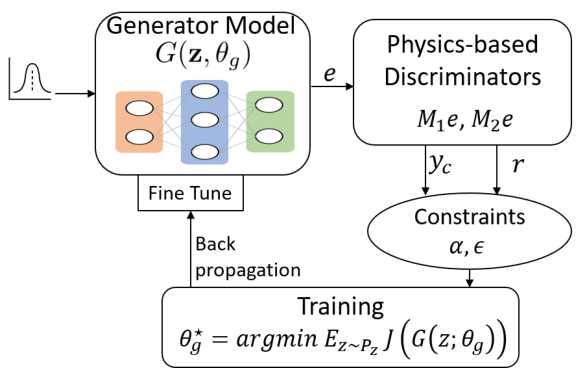
\includegraphics[scale=0.5]{image/GM.png}
    \caption{\textcolor{blue}{Physics-based generative model and training process ($\alpha$ is the lower-bound constraint for attack effectiveness while $\epsilon$ is the upper-bound constraint for attack stealthiness)}}
    \label{fig:GM}
\end{figure}
%%%%%%%% Use Generative model (GM) to generate elements of a set (Mathematical development)
The training process is shown in Fig.~\ref{fig:GM}. The output of the generator is passed, through the discriminator boundary functions, to a loss  function designed such that the weights of the generator network are trained to ensure that the outputs of the discriminators satisfy the constraints. Since the constraints are threshold-based, we use an indicator-like loss function:
\begin{equation}
    J(\mathbf{e}) = \textsf{ReLU}(\alpha - \|M_1\mathbf{e}\|_2)+\textsf{ReLU}(\|M_2\mathbf{e}\|_2 - \epsilon).
\end{equation}

Consequently, the generator is trained by solving the unconstrained optimization problem
\begin{align}\label{equ:training_GM}
    \boldsymbol{\theta}_g^* = \argmin\underset{\mathbf{z}\sim \textbf{P}_z}{\mathbb{E}}J(G(\mathbf{z};\boldsymbol{\theta}_g))
\end{align}
via back propagation.

\iffalse
{\color{red}\textbf{Please update Fig. 1 to reflect the description above. Specifically, replace the Loss Fun with the optimization problem above. Change "Loss Fun" to "training"}}
\fi







\section{Detection and Localization}\label{sec:detection_localization}
% Detection and localization (Ali)
% \begin{enumerate}
%     \item Definitions/description: Please clarify anomaly detection and localization separately. Detection is to identify if there is an attack on measurements. Localization requires to identify the location of attacks.
%      the term \texttt{attack location} refers to sensor channels (or indices) through which the attack signals are added to the system, and the term \texttt{localization} refers to the algorithmic process of estimating the attack location for a give CPS.
%     \item Describe the data generation process:
%     \begin{itemize}
%         \item randomize attack location 
%         \item GM generate \textcolor{blue}{FDIA} for that support 
%         \item Package the data to train a multi-class MLP as the initial localization: (get confidence) network structure, loss function, training algorithm
%         \item Attack pruning for improved resiliency: Bring results from previous papers 
%     \end{itemize}
% \end{enumerate}

%%%%%%% Definitions/description (Yu)
\iffalse
{\color{red}\textbf{A little motivation to connect this section to the previous one. We already have (Model Development) which built physics-based model for the discriminator in GM training  for (Automated Attack Generation). How does this section fit into that narrative? Use one or two simple very clear sentences for this.}}
\fi

Through an automated attack generation by a well-trained generative model, an adversarial training dataset could be \textcolor{blue}{generated} and used to improve the precision of the \textcolor{blue}{supervised learning-based} attack detection and localization algorithm. In this section, \textcolor{blue}{a detection and localization algorithm} is given by training a multi-layer perceptron (MLP) on the generated attack dataset. In addition, by analyzing the uncertainty \textcolor{blue}{of} the MLP's output, a pruning algorithm is proposed to improve the localization precision further.

The term \texttt{attack location} refers to sensor channels (or indices) through which the attack signals are added to the system. Let $\mathcal{T}$ denote the actual attack support, then we define its indicator element-wise as:
 \begin{equation} \label{equ:support}
     \mathbf{q}_i\left\{
     \begin{array}{lr}
     0 &\quad\text{if}\hspace{0.2cm} i \in \mathcal{T} \\
     1 &\quad\text{otherwise}.
     \end{array}
     \right.
 \end{equation}
 
 Next, the definitions of detection and localization are given:
 \begin{definition}[Detection]
Given a measurement vector $\mathbf{y} \in \mathbb{R}^m$, detection is a function $D:\mathbb{R}^m \rightarrow \{0,1\}$ whose output $D(\mathbf{y})$ indicates the existence of attack signal in the input $\mathbf{y}$.
 \end{definition}
 
 \begin{definition}[Localization]
 Given a measurement vector $\mathbf{y} \in \mathbb{R}^m$, localization is a function $L:\mathbb{R}^m \rightarrow \{0,1\}^m$ whose output indicates detection result for each measurement channel. In particular, \textcolor{blue}{it is an estimate $\hat{\mathcal{T}}$ of the actual attack support $\mathcal{T}$. Its indicator $\hat{\mathbf{q}}$ is defined similarly to \eqref{equ:support}, using $\hat{\mathcal{T}}$}
 \end{definition}

%%%%%%% Describe the data generation process:  
% 1. randperm to randomize attack location,  (Yu)

\iffalse
\begin{figure}
    \centering
    \includegraphics[scale=0.55]{MLP_training.png}
    \caption{Diagram of Training data generation process for multi-class MLP}
    \label{fig:MLP_training}
\end{figure}
\fi


% 2. GM generate \textcolor{blue}{FDIA} for that support (Yu)



% 3. Package the data to train a multi-class MLP as the localization algorithm: (get confidence) (Ali)
\iffalse
{\color{red}\textbf{This MLP section needs to be redone completely. Please connect with the paper. Currently, it reads like a class note. This is a research article. Do NOT write as if you are teaching the reader what MLP is. But write as we are applying MLP to the problem. So, the equations, language and training description should connect with the rest of the paper. Also eqn (19) seems incomplete. What is it? Please put in perspective. Specifically answer the following questions in your write up:}
\begin{itemize}
    \item What do we want to achieve and why is MLP a good choice?
    \item What is the equation that describe the input-output relationship of the particular MLP for this paper? --  Make the equation connect with the rest of the paper. For instance, it seems $f$ needs to be $\hat{\mathbf{q}}$?
    \item How is the training data generated. You need to describe this very simply and clearly.
    \item How will the trained MLP be used within the resilient algorithm suite?
\end{itemize}
}

Multilayer Perceptron (MLP) is used to detect \textcolor{blue}{FDIAs}. MLP is a special feed-forward neural networks where the information travels in one direction through all layers. It consists of several layers of nodes: an input layer, a hidden layer, and an output layer. MLPs are capable identifying high dimension non-linearly separable features. The output for a single perceptron in an MLP is given by: 
\begin{equation}
    f= \varphi (\sum_{i=1}^{n} w_is_i+b)\vspace{-0.07in},
\end{equation}
where $\varphi$ is the non-linear activation function, $f$ is the estimated output from the activation function, $w$ is the weight, $s_i$ is the input variable, $b$ is the bias, and $n$ is the input dimension. 
The activation function is a crucial feature of deep learning algorithms as it determines if and to what extent a neuron output should be considered. For this paper, Rectified linear unit (RELU), Sigmoid, and hyperbolic tangent are used \cite{glorot2010understanding}. Cross-entropy loss is utilized to evaluate the detection of the MLP classification and can be calculated as:  

% \hl{The training is done by searching for the parameters $w_{ji}$, $b_i$ that minimizes the experimental loss functional} 
\begin{equation} \label{equ:MLP_loss}
-\sum_{i=1}^{N}\:\: (y_i \log (p_i)+(1-y_i) \log (1-p_i))
\end{equation}

% \begin{equation}
%     F(\mathbf{\omega},b,\{\mathcal{S},\mathcal{Y}\}) = \sum\limits_{j=1}^{M_{Tr}}{\left(y_j-\varphi (\sum_{i=1}^{n} w_{ji}{s_j}_i+b_j)\right)^2}
% \end{equation}
\fi

\textcolor{blue}{As universal function approximators}, shown in Cybenko's theorem \cite{cybenko1989approximation}, MLPs are used to describe mathematical models via a regression scheme. Attack detection and localization is a multi-line binary classification task. With adequate training dataset generated by the automated attack generator, MLP's advantages of being a \textcolor{blue}{supervised} learning network could be fully utilized.

The MLP used in this paper is a three-layer neural network containing two \emph{LeakyReLU} hidden layers and one \emph{Sigmoid} output layer, and the final classification outputs are $0$ (for attack) if the corresponding MLP output is less than $0.5$, \textcolor{blue}{and $1$ (for no attack) otherwise}. The output layer's size is the same as the input size and equal to the number of attacks. Consequently, the MLP is given by
\begin{equation}\label{equ:MLP}
    g(\mathbf{y}; \boldsymbol{\theta}) \triangleq \phi \left(\sum_{i=1}^{n} w_i\mathbf{y}_i+b\right),
\end{equation}
where $\phi$ is the activation function of the output layer and $\boldsymbol{\theta}$ is a vector of tunable weights and biases.
Then, the localization output is given by
\begin{equation}\label{equ:classification}
    \hat{\mathbf{q}}_i=\left\{
     \begin{array}{lr}
     1 &\quad\text{if}\hspace{0.2cm} g({\mathbf{y}}_i;\boldsymbol{\theta})\geq 0.5 \\
     0 &\quad\text{otherwise}.
     \end{array}
     \right.
\end{equation}
  
Next, a supervised learning algorithm, via back propagation, is used to train the MLP \textcolor{blue}{using the} binary cross-entropy loss function:
\begin{align}\nonumber
    J(\boldsymbol{\theta}) &= \frac{1}{N}\sum_{i=1}^N\left( \mathbf{q}^{(i)}\log g({\mathbf{y}^{(i)}};\boldsymbol{\theta}) \right.\\\label{equ:MLP_loss}  
    &\hspace{1.5cm}\left. +(\mathbf{1}-\mathbf{q}^{(i)};\boldsymbol{\theta}) \log (\mathbf{1}-g({\mathbf{y}^{(i)}};\boldsymbol{\theta}))\right),
\end{align}
where $(\mathbf{y}^{(i)}, \mathbf{q}^{(i)})$ is the $i$th training data, and $N$ is the total number of data points.



%%%%%%%% Attack pruning for improved resiliency: Bring results from previous papers (Yu)
\iffalse
{\color{red}\textbf{There seems to be a disconnect from the MLP section. Start by motivating the need for uncertainty modeling. We need a brief discussion of the purpose of the pruning algorithm.}
\begin{enumerate}
    \item Why is uncertainty model needed? 
    \item What will the uncertainty model be used for? -- to develop the pruning algorithm
    \item Continue with the rest of the development and end with a very clear and concise description of how the pruning algorithm will be used in the resilient estimation.
    \item Since it is impossible to completely describe the pruning process here, refer the reader to our earlier paper on the topic and make sure what you have here is a good SUMMARY. Omit details like Lemma V.1. I know you used the lemma because of $\mathbf{r}(k)$ in the $l_\eta$ equation. You can just use where clause to state $\mathbf{r}(k)$ instead of the Lemma. The Lemma will make it difficult to follow the paper because there is no proof and readers cannot imagine the proof based on this paper -  a lot of missing ingredients.
\end{enumerate}
}
\fi
Since the MLP-based attack detection and localization method described above is a multi-line binary classification, the agreement between the localization result $\hat{\mathbf{q}}$ and the actual attack support $\mathbf{q}$ can be described by a Bernoulli distributed agreement variable $\epsilon_i \sim \mathcal{B}(1,\mathbf{p}_i)$ \textcolor{blue}{given by}
 \begin{equation} \label{equ:uncertainty_model}
     \mathbf{q}_i=\epsilon_i\hat{\mathbf{q}}_i+(1-\epsilon_i)(1-\hat{\mathbf{q}}_i),
 \end{equation}
 where $\mathbf{p}_i= \mathbb{E}[\epsilon_i] = \textsf{Pr}\left\{\epsilon_i = 1\right\}$ is the confidence of the localization algorithm at $i$ channel, which is often obtained by the true rate in \emph{Receiver Operator Characteristic} (ROC) of the algorithm. 
 
 \iffalse
 $\mathbf{q}, \hat{\mathbf{q}}$ are indicator of unknown actual support prior $\mathcal{T}$ and predicted support prior $\hat{\mathcal{T}}$ by localization algorithm respectively, defined element-wise as:
  \begin{equation} \label{equ:support}
     \mathbf{q}_{i}=\left\{
     \begin{array}{lr}
     0 &\quad\text{if}\hspace{0.2cm} i \in \mathcal{T} \\
     1 &\quad\text{otherwise}.
     \end{array}
     \right.,
     \hat{\mathbf{q}}_{i}=\left\{
     \begin{array}{lr}
     0 &\quad\text{if}\hspace{0.2cm} i \in \hat{\mathcal{T}} \\
     1 &\quad\text{otherwise}.
     \end{array}
     \right.
 \end{equation}
 \fi
 
Consequently, the precision of the resulting support prior indicator $\hat{\mathbf{q}}$ is defined as follows:
  \begin{definition}[Positive Prediction Value, Precision, $\textsf{PPV}$ \cite{fawcett2006introduction}]\label{Def:PPV_def}
Given an estimate $\hat{\mathbf{q}}\in\{0,1\}^{N}$ of an unknown attack support indicator $\mathbf{q}\in\{0,1\}^{N  }$, $\textsf{PPV}$ is the proportion of $\mathbf{q}$ that is correctly identified in $\hat{\mathbf{q}}$. It is given by
\begin{equation}\label{equ:PPV_def}
\textsf{PPV} =  \frac{\|\mathbf{q} \odot \hat{\mathbf{q}} \|_{0}}{\|\hat{\mathbf{q}}\|_{0}} .
\end{equation}
\end{definition}
 
 \iffalse
 \begin{lemma}(\cite{zheng2020attack})  \label{Lem:PBD_CDF}
Given mutually independent Bernoulli random variables $\epsilon_i \sim \mathcal{B}(1,\mathbf{p}_i)$, $i=1,\cdots,Tm$, then
  \begin{equation}\label{equ:PMF}
      \textsf{Pr}\left\{\sum_{i=1}^{Tm} \epsilon_{i} = k-1 \right\}=\mathbf{r}(k), k=1,\cdots,Tm+1
  \end{equation}
  where,
  $$ \mathbf{r} = \beta \cdot \begin{bmatrix}-\mathbf{s}_1\\1 \end{bmatrix} * \begin{bmatrix}-\mathbf{s}_2\\1 \end{bmatrix} * \cdots * \begin{bmatrix}-\mathbf{s}_{Tm}\\1 \end{bmatrix}
  $$
  with
  $ \beta =\displaystyle\prod_{i=1}^{Tm} \mathbf{p}_{i}, \hspace{2mm} \mathbf{s}_i = -\frac{1-\mathbf{p}_{i}}{\mathbf{p}_{i}}
  $
\end{lemma}
\fi

Next, with the attack localization result $\hat{\mathcal{T}}$, the estimated support of safe nodes can be represented as $\hat{\mathcal{T}}^c = \{j_1, j_2,\cdots, j_{|\hat{\mathcal{T}}^c|}\}$. A \emph{Pruning Algorithm} is proposed to prune the most \textcolor{blue}{probable} erroneous localization results in $\hat{\mathcal{T}}^c$. 

\noindent The first step is to obtain a trust \textcolor{blue}{length} $l_{\eta}(\leq Tm)$ based on the confidence of the localization results $\mathbf{p}$.  Given a reliability level $\eta \in (0,1)$, the trust \textcolor{blue}{length} $l_{\eta}$ is \textcolor{blue}{an integer} defined as the maximum number of safe nodes correctly localized in $\hat{\mathcal{T}}^c$ with a probability of at least $\eta$\textcolor{blue}{;}
\begin{equation}\label{equ:trust_number_def}
    l_{\eta} \triangleq \textsf{max} \left\{k \biggl\lvert \textsf{Pr} \left\{\sum_{i\in \hat{\mathcal{T}}^c} \epsilon_i \geq k \right\}\geq \eta \right\}.
\end{equation}
Let
\begin{equation} \label{equ:r_tau_hat_c}
    \bar{\mathbf{r}} \triangleq \begin{bmatrix}r_{0} \\ r_{1} \\\vdots \\ r_{|\hat{\mathcal{T}}^c|}\end{bmatrix} = \displaystyle\prod_{i=1}^{|\hat{\mathcal{T}}^c|} \mathbf{p}(j_i)  \begin{bmatrix}-s_{j_1}\\1 \end{bmatrix} * \begin{bmatrix}-s_{j_2}\\1 \end{bmatrix} * \cdots * \begin{bmatrix}-s_{j_{|\hat{\mathcal{T}}^c|}}\\1 \end{bmatrix},
\end{equation}
where $s_{j_i} = -\frac{1-\mathbf{p}_i}{\mathbf{p}_i}$.
Then, \textcolor{blue}{$\displaystyle\textsf{Pr}\left\{\sum_{i\in\hat{\mathcal{T}}^c} \epsilon_i = k\right\} = \bar{\mathbf{r}}_k$.}
Thus \eqref{equ:trust_number_def} becomes\footnote{\textcolor{blue}{$\displaystyle\textsf{Pr}\left\{\sum_{i \in \hat{\mathcal{T}}^{c}} \epsilon_{i} \leq k\right\} \leq 1-\eta$ is equivalent to $\displaystyle\textsf{Pr}\left\{\sum_{i \in \hat{\mathcal{T}}^{c}} \epsilon_{i} = 0\right\} + \textsf{Pr}\left\{\sum_{i \in \hat{\mathcal{T}}^{c}} \epsilon_{i} = 1\right\} +\cdots \textsf{Pr}\left\{\sum_{i \in \hat{\mathcal{T}}^{c}} \epsilon_{i} = k\right\} \leq 1-\eta$ since $k$ could only be integer.}}
\textcolor{blue}{
\begin{equation}\label{equ:trust_number}
\begin{aligned}
l_{\eta}&= \textsf{max} \left\{k \biggl\lvert \textsf{Pr}\left\{\sum_{i \in \hat{\mathcal{T}}^{c}} \epsilon_{i} \leq k\right\} \leq 1-\eta\right\}  \\
&= \textsf{max} \left\{k \biggl\lvert \sum_{i=0}^{k} \bar{\mathbf{r}}_i \leq 1-\eta \right\}.
\end{aligned}
\end{equation}}


\noindent The second step is to obtain a \emph{Pruned Support Prior} $\hat{\mathcal{T}}^{c}_{\eta}$ of size $l_{\eta}$\textcolor{blue}{. This is done through the robust extraction:}
\begin{equation}    \label{equ:pruning_alg}
    \hat{\mathcal{T}}^{c}_{\eta} =  \big\{\textsf{argsort} \downarrow (\mathbf{p} \odot g(\mathbf{y};\boldsymbol{\theta}))\big\}_{1}^{l_{\eta}},
\end{equation}
where $\{\cdot\}_{1}^{l_{\eta}}$ \textcolor{blue}{denotes} an index extraction from the first elements to $l_{\eta}$ elements. To obtain a pruned support prior consistent with the model assumptions in Section ~\ref{sec:system_model}, its size should satisfy $l_{\eta}\geq k_0$, where $k_0$ is a lower bound of $\hat{\mathcal{T}}^{c}_{\eta}$ such that $(A,C_{\hat{\mathcal{T}}^{c}_{\eta}})$ is observable. This can be guaranteed by the proper choice of the reliability level $\eta$, as given in the following theorem.
\begin{theorem}\label{Thm:eta_upper_bound}
Given a measurement redundancy preservation parameter $k_0>0$, the size of pruned support prior satisfies $l_{\eta}\geq k_0$ if
\begin{equation}\label{equ:eta_upper_bound}
\eta \leq  1- \sum_{i=0}^{|\hat{\mathcal{T}}^c|} e^{k_0-i} \bar{\mathbf{r}}_i,
\end{equation}
where $\bar{\mathbf{r}}$ is given by \eqref{equ:r_tau_hat_c}, and $\hat{\mathcal{T}}^c$ is the estimated support of safe nodes from the attack localization algorithm.
\end{theorem}
\begin{proof}
According to \eqref{equ:trust_number_def}, a sufficient condition for $l_{\eta} \geq k_0$ is
\begin{align*}
\textsf{Pr} \left\{\sum_{i\in \hat{\mathcal{T}}^c} \epsilon_{i} \geq k_0 \right\} &\geq \eta,
\end{align*}
which is equivalent to:
\begin{align*}
\textsf{Pr} \left\{k_0 - \sum_{i\in \hat{\mathcal{T}}^c} \epsilon_{i}  \leq 0 \right\}&\geq \eta
\end{align*}
and
\begin{align}
    \textsf{Pr} \left\{k_0-\sum_{i\in \hat{\mathcal{T}}^c} \epsilon_{i}  \geq 0 \right\}&\leq 1-\eta. \label{equ:trust_num_rewritte}
\end{align} 
According to Lemma~\ref{Lem:chance_constrain}, let $z = k_0-\sum_{i\in \hat{\mathcal{T}}^c} \epsilon_{i}$, and take $\Phi(z) = \exp(z)$ yields a sufficient condition for \eqref{equ:trust_num_rewritte} as
\begin{align} 
&\mathbb{E}\left[\exp\left(k_0-\sum_{i\in \hat{\mathcal{T}}^c} \epsilon_{i}\right)\right] \leq 1-\eta, \nonumber \\
\equiv\hspace{2mm}& e^{k_0}\mathbb{E}\left[\exp\left(-\sum_{i\in \hat{\mathcal{T}}^c} \epsilon_{i}\right)\right] \leq 1-\eta. \label{equ:sufficient_cond}
\end{align}
Since $\displaystyle\textsf{Pr}\left\{\sum_{i\in\hat{\mathcal{T}}^c} \epsilon_i = k\right\} = \bar{\mathbf{r}}_k$, it follows that
\begin{align}
    \mathbb{E}\left[\exp\left(-\sum_{i\in \hat{\mathcal{T}}^c} \epsilon_{i}\right)\right] &= \sum_{k =0}^{|\hat{\mathcal{T}}^c|} e^{-k}  \textsf{Pr}\left\{\sum_{i\in\hat{\mathcal{T}}^c} \epsilon_i= k\right\}\nonumber \\
    &= \sum_{k =0}^{|\hat{\mathcal{T}}^c|} e^{-k} \bar{\mathbf{r}}_k.  \label{equ:closed_form_expression}
\end{align}
 Combining \eqref{equ:sufficient_cond} and \eqref{equ:closed_form_expression} yields
\begin{equation}
    \sum_{i=0}^{|\hat{\mathcal{T}}^c|} e^{k_0-i} \bar{\mathbf{r}}_i\leq 1-\eta.
\end{equation}
Finally, an upper bound on $\eta$ is obtained as \eqref{equ:eta_upper_bound}.
\end{proof}
\begin{remark}\label{rmk:performance_require}
From \eqref{equ:eta_upper_bound}, it is clear that, necessarily, the upper bound should be strictly positive. This yields the following pruning requirement on the localization performance parameters:
\begin{align}\label{equ:localization_performance_criterion}
\sum\limits_{i=0}^{|\hat{\mathcal{T}}^c|}e^{-i}\bar{\mathbf{r}}_i < e^{-k_0}.
\end{align}
If this holds, according to the assumption $A2$, with at least $k_0$ safe nodes remaining in the pruned support prior $\hat{\mathcal{T}}^c_{\eta}$, $(A,C_{\hat{\mathcal{T}}^c_{\eta}})$ will be observable. Thus the asymptotic convergence of the estimation error is guaranteed. 
% Thus, the resilient $\ell_2$ observer designed on $(A,C_{\hat{\mathcal{T}}^c_{\eta}})$ can estimate the state variables correctly.
%{\color{red}We may need to check this property in the simulation section for the localization algorithm }{\color{blue}we would give theorem for the estimation error bound of resilient L2 for this concern. }{\color{red} A theorem is good. But we still need to check with the simulation. For example: What is $k_0$ for MLP1? }
\end{remark}

\iffalse
\begin{remark}{\color{red}Remove this. First see the corrected version above.}
According to \eqref{equ:eta_upper_bound}, it is clear that the preserved number of measurements $k_0$ through pruning has a upper bound $\sum_{i=0}^{|\hat{\mathcal{T}}^c|}\left(i-log\mathbf{r}_{\hat{\mathcal{T}}^c}(i+1)\right)$ which depends mainly on the attack localization result $\hat{\mathcal{T}}^c$. If $\hat{\mathcal{T}}^c$ covers more exact safe nodes in $\mathcal{T}^c$, then the upper bound is bigger. According to the assumption $A2$, with at least $k_0$ safe nodes remained in pruned support prior $\hat{\mathcal{T}}^c_{\eta}$, $(A,C_{\hat{\mathcal{T}}^c_{\eta}})$ is observable. 
% Thus, the resilient $\ell_2$ observer designed on $(A,C_{\hat{\mathcal{T}}^c_{\eta}})$ can estimate state variables correctly.
\end{remark}
\fi

\iffalse
For pragmatic reasons, it is important to ensure that $l_{\eta} >0$ in \eqref{equ:trust_number}. This is guaranteed if $\eta$ is chosen such that at least one node is selected into the pruned set. Formally, this condition is given by:
\begin{equation}\label{equ:condition_for_eta}
    \eta \leq \max_{i\in \hat{\mathcal{T}}^c}{(\mathbf{p}_i)}
\end{equation} 
\fi

\noindent Moreover, it was shown in \cite{zheng2021Resilient} that the precision $\textsf{PPV}_{\eta}$ of the pruned support prior $\hat{\mathcal{T}}^c_{\eta}$ given by \eqref{equ:pruning_alg} achieves
\begin{equation}\label{equ:precision_after_pruning}
    \textsf{Pr}\left\{\textsf{PPV}_{\eta} =1 \right\} \geq \eta.
\end{equation} 
This indicates that, with the probability of at least $\eta$, the measurement nodes contained in $\hat{\mathcal{T}}^c_{\eta}$ are all safe, and $(A,C_{\hat{\mathcal{T}}^c_{\eta}})$ is observable according to Remark~\ref{rmk:performance_require}. Thus, with the probability of at least $\eta$, \textcolor{blue}{exact state} estimation can be achieved by using $\ell_2$ observer designed based on $(A,C_{\hat{\mathcal{T}}^c_{\eta}})$.
Finally, \textcolor{blue}{Algorithm~\ref{Alg:ADL_AAG_P}} summarizes the attack detection and localization using automated attack generation and pruning operation.
\begin{algorithm}[h!]\label{Alg:ADL_AAG_P}
\SetAlgoLined
\uppercase\expandafter{\romannumeral1}.\hspace{2mm}\textbf{Offline: Dataset generation and training.}\\
\begin{enumerate}
    \item Given time horizon $T$, prepare $M_1, M_2$ matrices for physics-based \textcolor{blue}{discriminators} $\leftarrow$ \eqref{equ:M1}, \eqref{equ:M2}.
    \item Given the number of attacks $|\mathcal{T}|$, randomize attack support $\mathcal{T}$, and obtain its indicator $\mathbf{q}$ $\leftarrow$ \eqref{equ:support}.
    \item Given attack indexes $\alpha, \epsilon$, train the generative model (GM) by solving the optimization problem in \eqref{equ:training_GM}.
    \item Generate attack dataset $\{Y\}$ using the trained GM. Evaluate generated attack dataset via simulation.
    \item Return the effective subset of attack dataset as the training dataset $\{Y, \mathbf{q}\}$.
    \item Train the MLP in \eqref{equ:MLP} using the generated dataset $\{Y, \mathbf{q}\}$ via backpropagation.
\end{enumerate}

\uppercase\expandafter{\romannumeral2}.\hspace{2mm}\textbf{Online: Localization and pruning}\\
\begin{enumerate}
    \item Input real-time measurements $\mathbf{y}$, obtain the classification result $\hat{\mathbf{q}}$ $\leftarrow$ \eqref{equ:MLP}, \eqref{equ:classification};
    \item \textcolor{blue}{Obtain} the pruned support prior $\hat{\mathcal{T}}^{c}_{\eta} (\hat{\mathbf{q}}_{\eta})$ $\leftarrow$ \eqref{equ:trust_number}, \eqref{equ:pruning_alg}.
\end{enumerate}

\textbf{Output}: $\hat{\mathcal{T}}^{c}_{\eta}$ (pruned support prior)
\caption{Attack detection and localization with automated attack generation and pruning}
\end{algorithm}

\section{Resilient Estimator}\label{sec:resilient_estimator}
%%%%%%%%%%% Resilient Kalman filter on the pruned safe sensor subset %%%%%%
In this section, the Kalman filter of Section~\ref{sec:system_model} is redesigned on the pruned safe support produced by Algorithm~\ref{Alg:ADL_AAG_P}, in order to maintain secure state estimation under FDIAs. The scheme is shown in Fig.~\ref{fig:resilient_L2_observer}: attack detection/localization returns an estimate $\hat{\mathcal{T}}^c$ of the safe sensors; pruning downselects the most trustworthy subset $\hat{\mathcal{T}}^c_{\eta}$; the resilient KF then updates using only $\mathbf{y}_{\hat{\mathcal{T}}^c_{\eta}}$, with the corresponding output matrix $C_{\hat{\mathcal{T}}^c_{\eta}}$ and noise covariance $R_{\hat{\mathcal{T}}^c_{\eta}}$.

\begin{figure}[h!]
    \centering
    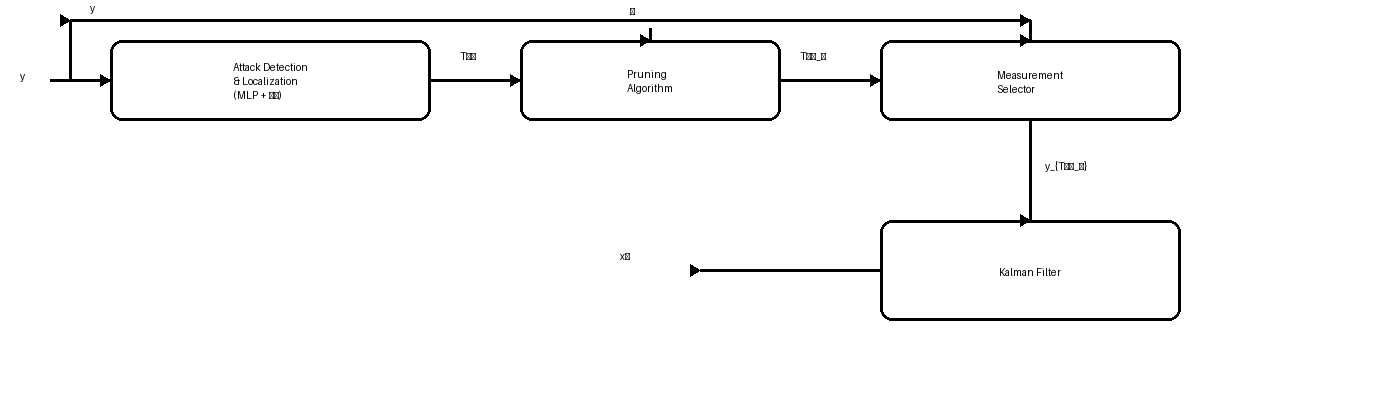
\includegraphics[width=\columnwidth]{image/resilient_L2_observer.png}
    \caption{Schematic diagram of the resilient Kalman filter with chi-square monitoring and support pruning}
    \label{fig:resilient_L2_observer}
\end{figure}

\subsection{Resilient Kalman filter}
Given $\hat{\mathcal{T}}^c_{\eta}$ at time $i$, the resilient KF uses the reduced measurement model
\begin{equation}\label{equ:reduced_meas}
\mathbf{y}_{\hat{\mathcal{T}}^c_{\eta},i}
=C_{\hat{\mathcal{T}}^c_{\eta}}\mathbf{x}_i+\mathbf{v}_{\hat{\mathcal{T}}^c_{\eta},i}+\mathbf{e}_{\hat{\mathcal{T}}^c_{\eta},i},
\end{equation}
and applies \eqref{equ:kf_predict}--\eqref{equ:kf_Pupdate} with $(C,R)$ replaced by $(C_{\hat{\mathcal{T}}^c_{\eta}},R_{\hat{\mathcal{T}}^c_{\eta}})$. Denote the resulting filtered estimate and covariance by $\hat{\mathbf{x}}_i'$ and $P_{i|i}(\hat{\mathcal{T}}^c_{\eta})$. By \eqref{equ:precision_after_pruning}, $\mathbf{e}_{\hat{\mathcal{T}}^c_{\eta},i}=\mathbf{0}$ with probability at least $\eta$.

When $|S|\ge k_0$ and $(A,C_S)$ is observable, the subset KF admits a unique stabilizing steady-state predicted covariance $P^-(S)\succ 0$ solving the DARE for $(A,C_S,Q,R_S)$, with filtered covariance
\begin{align}
P_{\infty}(S)&=(I-K(S)C_S)P^-(S), \label{equ:Pinf}\\
K(S)&=P^-(S)C_S^{\top}\big(C_SP^-(S)C_S^{\top}+R_S\big)^{-1}. \nonumber
\end{align}
The map $S\mapsto \mathrm{tr}\,P_{\infty}(S)$ is monotonically nonincreasing under set inclusion: if $S_1\subset S_2$ and both satisfy A2, then $\mathrm{tr}\,P_{\infty}(S_2)\le \mathrm{tr}\,P_{\infty}(S_1)$ \cite{anderson2012optimal}. This yields the graded estimation-error link in the sparsity--observability--precision chain.

\begin{theorem}[Resilient KF performance]\label{Thm:resilient_estimation_gaurentee}
Let $\hat{\mathcal{T}}^c_{\eta}$ be given by \eqref{equ:pruning_alg}, and suppose $\eta$ satisfies \eqref{equ:eta_upper_bound} with the localization performance criterion \eqref{equ:localization_performance_criterion}. Then, with probability at least $\eta$,
\begin{enumerate}
\item[(i)] $\mathbf{e}_{\hat{\mathcal{T}}^c_{\eta}}=\mathbf{0}$ and $|\hat{\mathcal{T}}^c_{\eta}|\ge k_0$, so $(A,C_{\hat{\mathcal{T}}^c_{\eta}})$ is observable;
\item[(ii)] the resilient KF coincides with the attack-free KF on the same sensor subset, and its steady-state mean-square error satisfies
\begin{equation}\label{equ:error_bound}
\lim_{i\to\infty}\mathbb{E}\big\|\hat{\mathbf{x}}_i'-\mathbf{x}_i\big\|_2^2
=\mathrm{tr}\,P_{\infty}(\hat{\mathcal{T}}^c_{\eta});
\end{equation}
\item[(iii)] relative to the full-sensor attack-free KF,
\begin{equation}\label{equ:error_gap}
\mathrm{tr}\,P_{\infty}(\{1,\ldots,m\})
\le
\mathrm{tr}\,P_{\infty}(\hat{\mathcal{T}}^c_{\eta})
\le
\mathrm{tr}\,P_{\infty}(S_{k_0}),
\end{equation}
for every observable subset $S_{k_0}$ of size $k_0$ that can arise from pruning at reliability $\eta$.
\end{enumerate}
\end{theorem}
\begin{proof}
Claim~(i) follows from \eqref{equ:precision_after_pruning}, Theorem~\ref{Thm:eta_upper_bound}, and assumption~A2. On that event the reduced measurements equal the attack-free subset measurements, so the KF recursions---and hence the limiting covariance \eqref{equ:Pinf}---coincide with the attack-free subset filter, which is claim~(ii). Claim~(iii) is the standard information monotonicity of the Riccati map under additional measurements, together with the worst-case size-$k_0$ subset admitted by the pruning length constraint.
\end{proof}

\begin{corollary}[Bridge summary]\label{Cor:bridge}
For attack sparsity $k$, observability threshold $k_0$, and localization confidences $\{\mathbf{p}_i\}$, Propositions~\ref{Prop:sparsity_observability}--\ref{Prop:precision_observability} and Theorem~\ref{Thm:resilient_estimation_gaurentee} jointly imply: every $\eta\in(0,\eta^{\star}]$ yields a pruned set that is clean and observable with probability $\ge\eta$, and the KF error is then exactly $\mathrm{tr}\,P_{\infty}(\hat{\mathcal{T}}^c_{\eta})$, sandwiched between the full-sensor and worst $k_0$-sensor Riccati costs. Thus sparsity constrains feasible $(k,k_0)$, precision $\eta$ trades against set size (hence against $\mathrm{tr}\,P_{\infty}$), and estimation error is quantitatively tied to both.
\end{corollary}

The chi-square monitor \eqref{equ:chisq_detector} may still be evaluated on the innovation of the resilient KF (with $S_i$ computed from $C_{\hat{\mathcal{T}}^c_{\eta}}$) to provide an online global alarm, while the MLP+pruning path supplies the channel support required by \eqref{equ:error_bound}--\eqref{equ:error_gap}.


\section{Simulation}\label{sec:simulation}
In this section, the resiliency improvement due to automated attack generation is shown in simulation by implementing Algorithm~\ref{Alg:ADL_AAG_P} and the resilient Kalman filter of Theorem~\ref{Thm:resilient_estimation_gaurentee} on a water distribution system. The experiments also illustrate the sparsity--observability--precision--error bridge of Corollary~\ref{Cor:bridge}.

\begin{figure}[!ht]
    \centering
    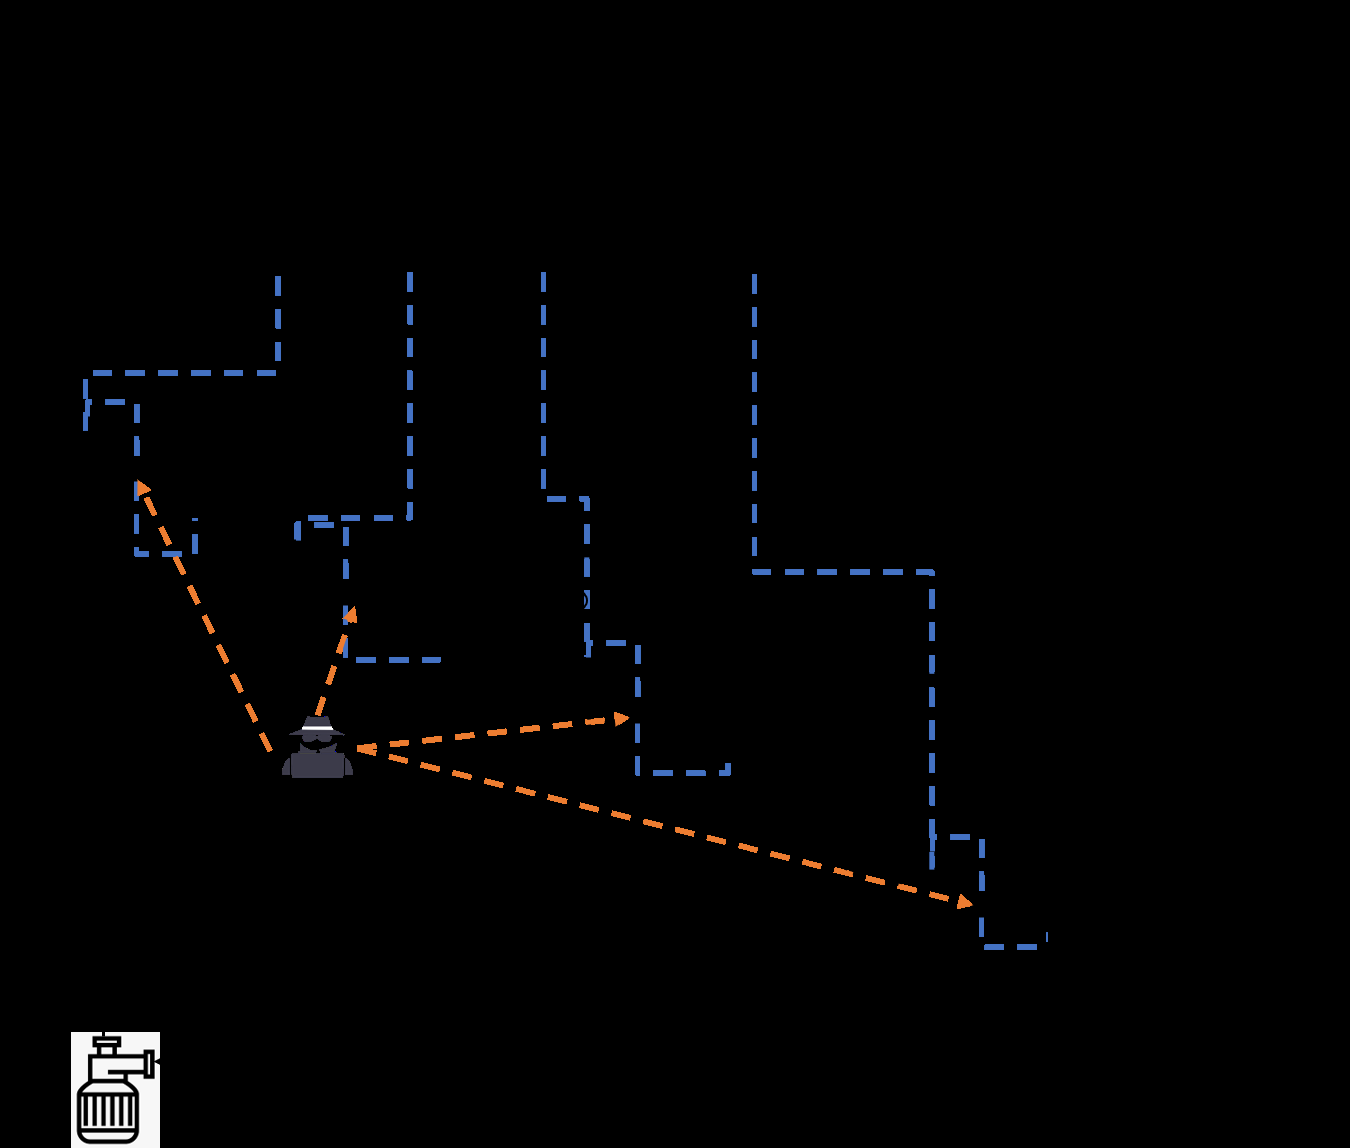
\includegraphics[width=\columnwidth]{image/WDS.png}
    \caption{Block diagram depiction of a water distribution system under \textcolor{blue}{FDIAs} (black solid are water pipelines, blue dotted lines are wireless data transmission lines for sensors data and control commands, orange dotted lines are attack injection route)}
    \label{fig:water_distribution_sys}
\end{figure}

The water distribution system, shown in Fig.~\ref{fig:water_distribution_sys}, contains $10$ distributed operating tanks and $1$ storage tank. The goal is to regulate all operating tanks' water levels around desired values. The magnetic valves $V_1 - V_{10}$ at the \textcolor{blue}{inlet} of operating tanks are controlled to adjust the water level of water tanks, and the manual valves $M_1 - M_{10}$ can be manipulated, at the demand point, to use the water from the corresponding tanks. The effect of these valves is modelled as the random demands $\mathbf{d}$ in \eqref{equ:water_level_adjustment}. The valves at the storage tank are fixed at a constant opening value.
\textcolor{blue}{For each operating tank, two sensors-water level meter and pressure sensors} ($L_1 ~ L_{10}$), are installed. The pressure sensors measure the difference of water level between adjoining tanks. The \textcolor{blue}{water levels} adjustment process is approximated by the LTI model:
\begin{equation}\label{equ:water_level_adjustment}
\begin{aligned}
   \mathbf{x}_{i+1} &= A\mathbf{x}_i + B\mathbf{u}_i - \mathbf{d}_i,\\
    \mathbf{y}_i &= C\mathbf{x}_i +\mathbf{v}_i + \mathbf{e}_i.
\end{aligned}
\end{equation}
where, $\mathbf{x}, \mathbf{u} \in \mathbb{R}^{10}$, \textcolor{blue}{$\mathbf{y}, \mathbf{v} \in \mathbb{R}^{61}$} are vector of water level, control input of magnetic valves, sensor measurements, and measurement noise respectively, $\mathbf{d} \in \mathbb{R}^{10}$ is the vector of random demands, and \textcolor{blue}{$\mathbf{e} \in \mathbb{R}^{61}$} is the injected \textcolor{blue}{FDIAs}. \textcolor{blue}{For the sake of clean presentation, interested readers are directed to \url{https://github.com/ZYblend/Resilient_WDS_AutoAttackGen} for the values of system parameters $A \in \mathbb{R}^{10\times 10},B \in \mathbb{R}^{10\times 10},C \in \mathbb{R}^{61\times 10}$.} Given \textcolor{blue}{a desired} water level $\mathbf{x}_d = 0.5 * \mathbf{1}_{10}$, \textcolor{blue}{the} proportional controller \textcolor{blue}{below} is used\textcolor{blue}{;}
$$ \mathbf{u}_i = -K(\hat{\mathbf{x}}-\mathbf{x}_d)-B^{-1}(A-I_{10})\mathbf{x}_d.
$$ 
The critical measurement in this scenario is the sum of all water levels of operating tanks, thus, the critical measurement matrix is given by $C_c = [1 \hspace{2mm} 1 \hspace{2mm} \cdots \hspace{2mm} 1] \in \mathbb{R}^{1\times 10}$. \textcolor{blue}{Firstly, a simulation experiment is done to assess the observability of the simulated system in order to obtain the least number of measurements from which the system states are fully observable. A Monte Carlos experiment, with $50000$ samples of randomly selected measurement subsets $\mathcal{S}$, is performed to calculated the probability of full observerability of $(A,C_{\mathcal{S}})$ using $|\mathcal{S}|$. Fig~\ref{fig:observability} shows that full observerability is preserved with $k_0 \geq 42$, corresponding to at most $30\%$ pruned measurements.}

\begin{figure}
    \centering
    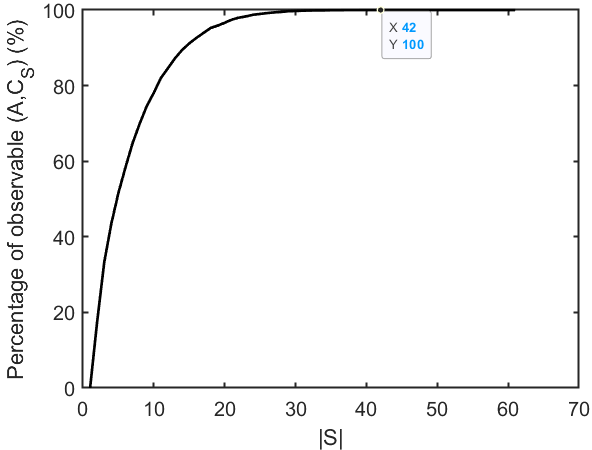
\includegraphics[scale=0.45]{new_sim_image/observability.png}
    \caption{\textcolor{blue}{Observability of simulated systems. The percentage of observable $(A,C_{\mathcal{S}})$ is calculated as the ratio of the number of observable $(A,C_{\mathcal{S}})$ to the total number of samples (=50000).}}
    \label{fig:observability}
\end{figure}

Next, we execute automated attack generation (against the KF/$\chi^2$ pair), MLP training, and Monte-Carlo simulation of the resilient KF under different detection/localization strategies.

\subsection{Automated attack generation}

A fixed time step of $T_s = 0.01s$ is used and the moving-window size is set as $T = 8T_s$. With different numbers of attacks, the discriminator maps $M_1$ (critical-output effectiveness through the KF--controller loop) and $M_2$ (chi-square stealthiness) are assembled for each random attack support. The generator in \eqref{equ:training_GM} is then trained as in Fig.~\ref{fig:GM}. Due to measurement noise and random demands, the thresholds are chosen as $\alpha = 0.1$ and $\epsilon=0.5$ (with $\epsilon$ aligned to the design chi-square level). Fig.~\ref{fig:train_result} shows effectiveness and the stealthiness statistic of generated attacks during training relative to $(\alpha, \epsilon)$. The trained generator maps uniform inputs to feasible attacks in \eqref{equ:success_FDIA_set}.
\begin{figure}[!h]
    \centering
    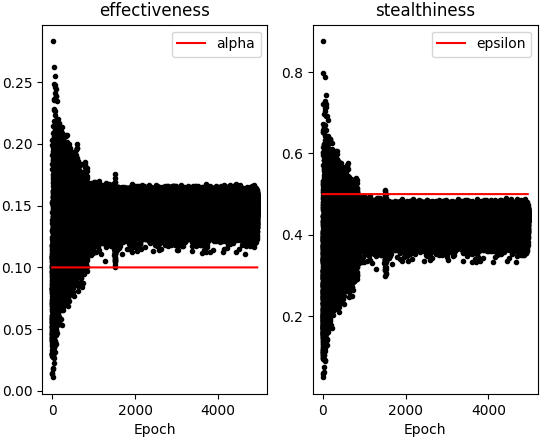
\includegraphics[scale=0.6]{new_sim_image/training_result.png}
    \caption{Feasibility of generated attacks during training. $\epsilon$ upper-bounds the chi-square stealthiness statistic $\|M_2 e\|_2$; $\alpha$ lower-bounds KF--controller effectiveness $\|M_1 e\|_2$.}
    \label{fig:train_result}
\end{figure}

\textcolor{blue}{The trained generator is then used to generate a dataset $D_\mathcal{S}(\alpha,\epsilon)$ of attacks. In order to inject the generated attacks, recursive feasibility \cite{lofberg2012oops} should be considered. An online moving-horizon attack injection scheme used here is to solve the following sample-based optimization program at each time step $i$: 
\begin{equation} \label{equ:attack_injection}
\begin{aligned}
       \displaystyle\Maximize_{\mathbf{e}_i} \hspace{2mm} &\left\|M_1 \begin{bmatrix}\mathbf{e}^{-} \\ \mathbf{e}_i\end{bmatrix}\right\|_2 \\
    \textsf{Subject to:} \hspace{2mm} & \left\|M_2 \begin{bmatrix}\mathbf{e}^{-} \\ \mathbf{e}_i\end{bmatrix}\right\|_2 \leq \epsilon \\
    & \mathbf{e}_i \in D_\mathcal{S}(\alpha,\epsilon)
\end{aligned}
\end{equation}
where $\mathbf{e}^{-}$ is the attack history during the time window $I^{-} = [i-T+1, i-1]$. Fig.~\ref{fig:generator_test_example_1} shows the performance of the generated attacks under the injection program \eqref{equ:attack_injection}.} The left panel shows that the windowed chi-square / innovation statistic under attack stays close to the nominal (attack-free) trajectory, i.e., the attacks remain stealthy relative to \eqref{equ:chisq_detector}. The right panel shows a clear deviation of the critical measurement, confirming effectiveness through the KF--controller loop.
\begin{figure}[!h]
    \centering
    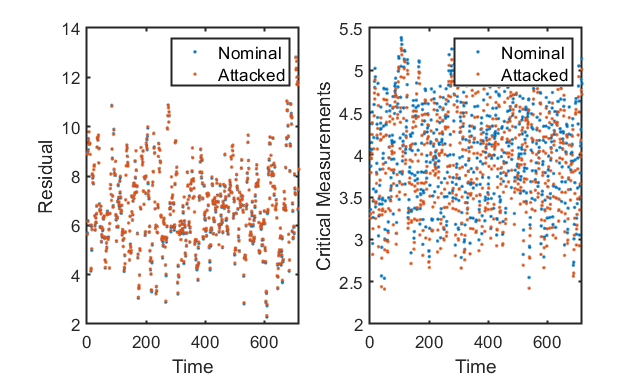
\includegraphics[width=\columnwidth]{new_sim_image/attack_effect.png}
    \caption{Performance of generated attacks injected through $39\%$ measurement nodes. (Left: windowed innovation / chi-square stealthiness statistic; Right: critical measurement.)}
    \label{fig:generator_test_example_1}
\end{figure}

 \textcolor{blue}{Next, the above automated attack generation scheme is trained to generate different types of attacks including different attack supports and different number of attacks. The generated attacks are then used to train the supervised learning-based attack detection and localization algorithm in next subsection.}

\subsection{MLP training}
To show one of the merits of the proposed automated attack generation scheme, two training datasets are prepared: one produced by random additive signals on measurements and the other augments the dataset with attack samples generated by the trained generator. Next, two MLP classifiers are trained on two datasets respectively. \textcolor{blue}{MLP1 and MLP2 are both four-layer fully-connected neural network with three "relu" hidden layers of $512, 1024, 512$ neurons respectively.  The output layer has $61$ neurons and uses "sigmoid" activation function. MLP1 is trained by the first random attack dataset, while MLP2 is trained the second training dataset containing automated generated attacks. The testing F1 score and precision of MLP1 are $85.1\%$ and $99.7\%$ respectively, while MLP2 achieves $88.7\%$ and $99.1\%$ respectively. The testing datasets used is $10\%$ of the corresponding datasets, so the testing datasets for MLP2 and MLP1 are different. Next, we compare the localization precision of the two MLPs on a same testing dataset which is an equal mixture of dataset 1 and dataset 2. As shown in Fig.~\ref{fig:MLP_compare}, MLP2 has successfully shifted the localization precision to the right, indicating a better performance overall. However, MLP1's performance is nearly uniform for different localization precision higher than $0.5$. This is because it is trained by random attack dataset. The mean precision of MLP1 is $74.37\%$, and the mean precision of MLP2 is $98.69\%$ on a testing set of successful \textcolor{blue}{FDIAs}.}   

\begin{figure}[!ht]
    \centering
    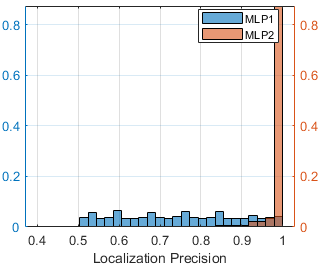
\includegraphics[scale=0.8]{new_sim_image/MLP_compare.png}
    \caption{\textcolor{blue}{A sample-based comparison of the performance of two MLP classifiers on same testing set of successful FDIAs. (MLP1: trained only with random attack generation, MLP2: trained with random attack generation and the proposed automated attack generation, $50000$ test cases are used.)}}
    \label{fig:MLP_compare}
\end{figure}

\begin{figure}[!ht]
    \centering
    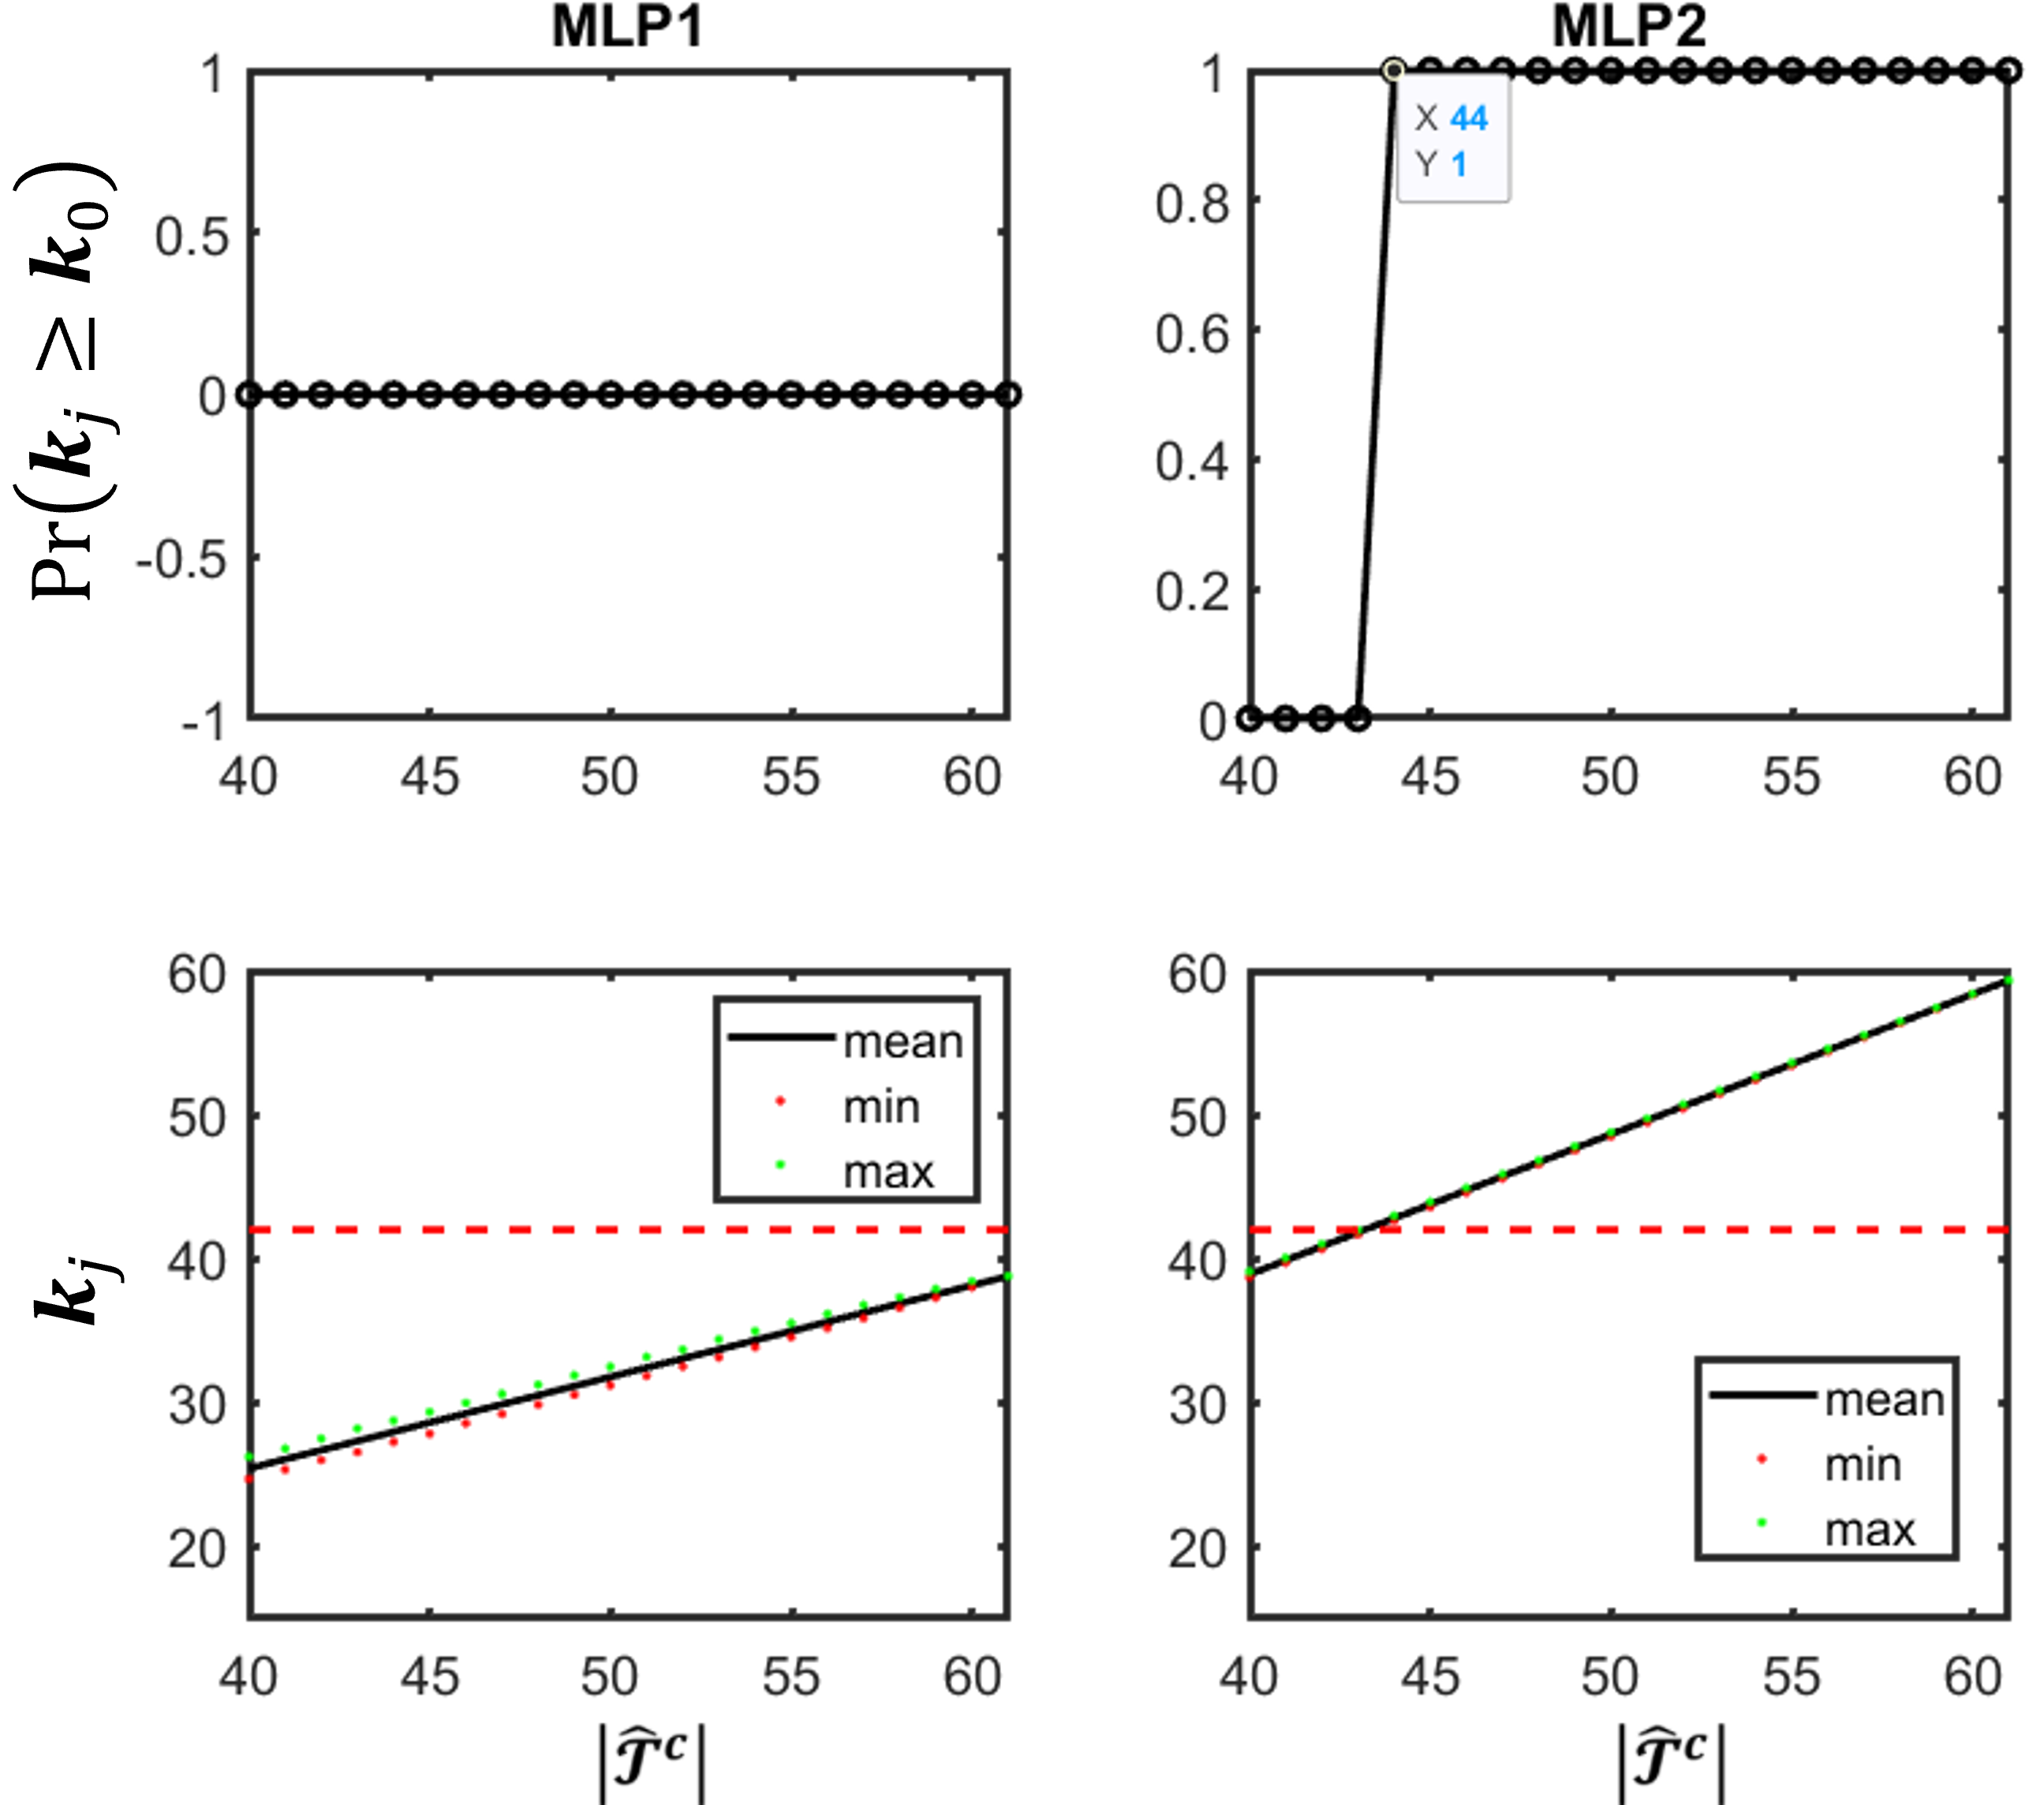
\includegraphics[scale=0.4]{new_sim_image/post_pruning_observability.png}
    \caption{\textcolor{blue}{A sample-based comparison of post-pruning observability for MLP1 and MLP2. ($50000$ test cases are used. The y axis for the top two subplots $Pr(k_j\geq k_0)$ is the sample estimate of the probability of at least $k_0$ measurements remaining after pruning. The black lines in the bottom subplots show the mean value of $k_j$ that is the number of measurements remaining after pruning, while the red and green dots are the minimum and maximum values of $k_j$'s respectively.}}
    \label{fig:MLP_compare_k0}
\end{figure}

As shown in Fig.~\ref{fig:observability}, full observability can be guaranteed with certainty if \textcolor{blue}{$k_0\geq 42$} measurements remains after pruning. For this, we evaluate the sufficient condition in \eqref{equ:localization_performance_criterion} on MLP1 and MLP2. First, the two MLPs are run on $10000$ cases generated by the trained generative model. From the results, the confidence vectors of the MLPs are estimated by calculating the true rates at all $61$ measurement nodes; for node $i$, $\mathbf{p}_i=\frac{TP_i+TN_i}{P_i+N_i}$. 
\iffalse
The confidence vectors of MLP1 and MLP2 are
$$\begin{aligned}
   &\mathbf{p}(\text{MLP1}) = [0.7076, 0.7065, 0.6883, 0.6621, 0.6855, 0.6790,\\
   &0.6721, 0.6807, 0.6623, 0.6791, 0.7535, 0.7610, 0.7519, 0.7334, \\
   &0.7692, 0.8001, 0.7393, 0.7150, 0.7667, 0.7519, 0.7544, 0.7338, \\
   & 0.7402, 0.7362, 0.7759, 0.7418, 0.7474, 0.7382, 0.7476, 0.7831, \\
   &0.7446, 0.7645, 0.7742, 0.7378, 0.7938, 0.7652, 0.7635, 0.7771, \\
   &0.7633, 0.7646],
\end{aligned} 
$$
$$\begin{aligned} &\mathbf{p}(\text{MLP21}) = [0.9826, 0.9819, 0.9828, 0.9853, 0.9866, 0.9737,\\
   &0.9804, 0.9858, 0.9748, 0.9749, 0.7692, 0.7685, 0.7764, 0.7855, \\
   &0.7667, 0.7995, 0.7422, 0.7528, 0.7729, 0.7959, 0.7631, 0.7996, \\
   & 0.7870, 0.7581, 0.7899, 0.7533, 0.7801, 0.8237, 0.7883, 0.8227, \\
   &0.7664, 0.7772, 0.8087, 0.8039, 0.8226, 0.8470, 0.8157, 0.8443, \\
   &0.8044, 0.8257].
\end{aligned} $$
\fi
Next, a sample based experiment is performed. For each support size \textcolor{blue}{$|\hat{\mathcal{T}}_j^c| \in \left\{40,41,\hdots,61\right\}$}, we generated  $\min\left\{^{61}C_{|\hat{\mathcal{T}}_j^c|},50000\right\}$ unique supports $\hat{\mathcal{T}}^c$, and  evaluated the right hand side of \eqref{equ:localization_performance_criterion} for each unique support as follows: 
$$k_j = -\ln\left(\sum_{i=0}^{|\hat{\mathcal{T}}_j^c|}e^{-i}\bar{\mathbf{r}}_i\right),$$
where the Poisson-binomial probability density vector $\bar{\mathbf{r}}_i$ is calculated, using the confidence vectors of \textcolor{blue}{the corresponding MLP}, based on \eqref{equ:r_tau_hat_c}. For each \textcolor{blue}{$|\hat{\mathcal{T}}_j^c| \in \left\{40,41,\hdots,61\right\}$}, and each MLP, the sample probability of the event $k_j\ge k_0$ and the expected value of $k_j$ are shown in Fig.~\ref{fig:MLP_compare_k0}. The results show that  MLP2 has a bigger chance of preserving post-pruning observability. Indeed, according to the figure, post-pruning observability cannot be guaranteed when MLP1 is used. \textcolor{blue}{In addition, from the bottom plots in Fig.~\ref{fig:MLP_compare_k0}, it is seen that MLP2 reduces the uncertainty on the post-pruning observability compared to MLP1.} By considering the sample-based analysis in Fig.~\ref{fig:MLP_compare} and Fig.~\ref{fig:MLP_compare_k0} together, it is seen that MLP performs better \textcolor{blue}{when trained with data generated by} the proposed automated attack generation.

Next, we compare MLP1 and MLP2 inside the resilient KF scheme.

\subsection{Resilient Kalman filter}
The trained MLPs, with and without pruning, are embedded in the real-time WDS simulation with the resilient KF of Section~\ref{sec:resilient_estimator}. A Monte-Carlo experiment estimates: (1)~the \textbf{probability of sustaining normal operation} (pSNO)---the fraction of times the critical-measurement deviation stays below a threshold; (2)~the \textbf{probability of triggering an alarm} (pTA)---the fraction of times the chi-square / innovation statistic exceeds its attack-free baseline by a threshold. Larger pSNO and pTA indicate better resiliency.

Attacks with sparsity from $1$ to $30$ are considered (five random-support scenarios each). For each detector variant (MLP1, MLP1+pruning, MLP2, MLP2+pruning), the pipeline in Fig.~\ref{fig:resilient_L2_observer} is simulated. Let $g_I$ denote the windowed chi-square statistic and $\mathbf{y}_{c_{i+1}}$ the critical output. Normalized deviations
$$\begin{aligned}
    \Delta g &= \frac{\left|(g_{I}-g_d)-(g^{\star}_{I} - g_d)\right|}{\textsf{max}\left(\left|(g_{I}-g_d)-(g^{\star}_{I} - g_d)\right|\right)}, \\
\Delta \mathbf{y} &= \frac{\left|(\mathbf{y}_{c_{i+1}}-\mathbf{y}_{c_d})-(\mathbf{y}^{\star}_{c_{i+1}}-\mathbf{y}_{c_d})\right|}{\textsf{max}\left(\left|(\mathbf{y}_{c_{i+1}}-\mathbf{y}_{c_d})-(\mathbf{y}^{\star}_{c_{i+1}}-\mathbf{y}_{c_d})\right|\right)},
\end{aligned}
$$
are formed relative to the attack-free noise-free baselines $g_d$ and $\mathbf{y}_{c_d}=C_c\mathbf{x}_d$. Then
$\mathrm{pTA}=\tfrac{1}{N}\|\Delta g \ge \tau_1\|_{\ell_0}$ and
$\mathrm{pSNO}=\tfrac{1}{N}\|\Delta \mathbf{y}\le \tau_2\|_{\ell_0}$,
with $\tau_1=1\%$ and $\tau_2=3\%$ calibrated on attack-free runs. These metrics empirically probe Corollary~\ref{Cor:bridge}: as sparsity $k$ grows, preserving $|\hat{\mathcal{T}}^c_{\eta}|\ge k_0=42$ and high $\textsf{PPV}_{\eta}$ becomes harder, which appears as degraded pSNO/pTA unless localization (MLP2) is strong enough.

\begin{figure}[!ht]
    \centering
    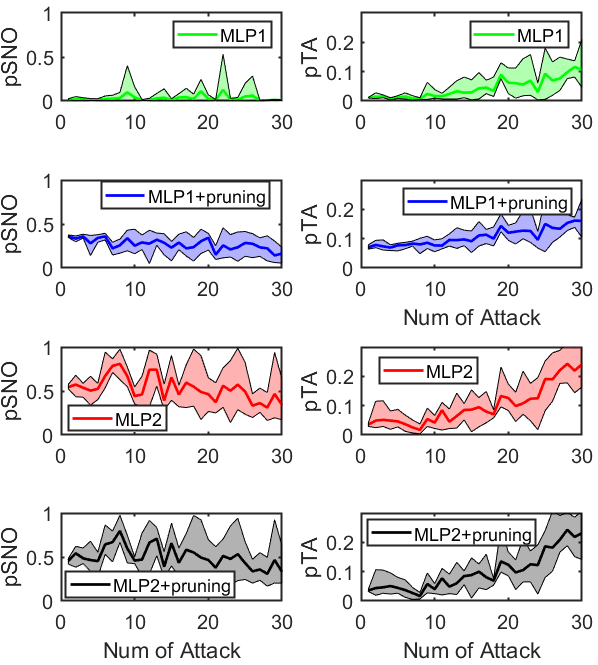
\includegraphics[scale=0.5]{new_sim_image/resiliency_compare.png}
    \caption{Resilient KF performance under different attack detection strategies; larger pSNO and pTA indicate better resiliency. Solid lines are means; shaded regions indicate spread.}
    \label{fig:resiliency_compare}
\end{figure}

Fig.~\ref{fig:resiliency_compare} compares pSNO and pTA across strategies. MLP2 outperforms MLP1 (and even MLP1+pruning), showing the value of generator-augmented training. Mean localization precision \eqref{equ:PPV_def} versus number of attacks is shown in Fig.~\ref{fig:precision}. Pruning still raises MLP2 precision, but state-estimation gains saturate once the observability budget $k_0$ binds---consistent with the $\eta$--$l_{\eta}$--$\mathrm{tr}\,P_{\infty}$ trade-off in Proposition~\ref{Prop:precision_observability} and Theorem~\ref{Thm:resilient_estimation_gaurentee}. MLP2+pruning nevertheless tightens the spread of pSNO/pTA, i.e., reduces performance uncertainty.


\begin{figure}[!ht]
    \centering
    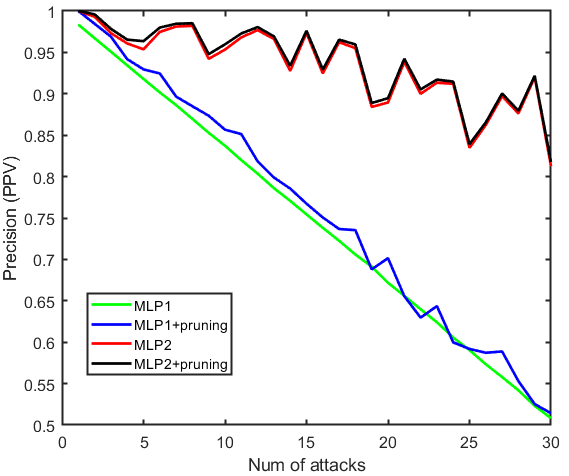
\includegraphics[scale=0.5]{new_sim_image/precision_vs_num_attack.png}
    \caption{\textcolor{blue}{A comparison of the mean precision of different attack detection strategies in the system simulation versus different number of attacks}}
    \label{fig:precision}
\end{figure}

\iffalse
\begin{table}[]
    \centering
    \caption{Mean value of attack localization precision}
    \begin{tabular}{|c|c|c|c|c|}
    \hline
       $\#$(attacks) & MLP1 & MLP1+pruning & MLP2 & MLP2+pruning  \\
        \hline 
       2  &  0.9150 & 0.9696 & 0.9559 & 0.9993\\
       3 & 0.8853 & 0.9427 & 0.9282 & 0.9790\\
       4 & 0.8612 & 0.9182 & 0.8998 & 0.9536\\
       5 & 0.8356 & 0.8925 & 0.8778 & 0.9381 \\
       6 & 0.8148 & 0.8651 & 0.8645 & 0.9201 \\
       7 & 0.7903 & 0.8414 & 0.8402 & 0.8878 \\
       8 & 0.7672 & 0.8116 & 0.8234 & 0.8823 \\
       9 & 0.7434 & 0.7905 & 0.7993 & 0.8677 \\
       10 & 0.7150 & 0.7602 & 0.7719 & 0.8407 \\
       11 & 0.6905 & 0.7377 & 0.7501 & 0.8296 \\
       12 & 0.6651 & 0.7091 & 0.7174 & 0.7904 \\
       13 & 0.6441 & 0.6851 & 0.7011 & 0.7689 \\
       14 & 0.6167 & 0.6598 & 0.6705 & 0.7496 \\
       15 & 0.5704 & 0.6349 & 0.6517 & 0.7388\\
       16 & 0.5704 & 0.6106 & 0.6412 & 0.7223\\
       17 & 0.5462 & 0.5833 & 0.6135 & 0.6955 \\
       18 & 0.5251 & 0.5576 & 0.5983 & 0.6751 \\
       19 & 0.5012 & 0.5305 & 0.5641 & 0.6265 \\
       20 & 0.4725 & 05069 & 0.5296 & 0.6192\\
       \hline
    \end{tabular}
    \label{tab:precision_table}
\end{table}
\fi


Finally, Fig.~\ref{fig:time_domain_result} shows a time-domain comparison under the same $39\%$ compromised measurements as in Fig.~\ref{fig:generator_test_example_1}. Schemes using MLP2 (with or without pruning) reduce critical-output deviation (smaller $\Delta \mathbf{y}$) while increasing the chi-square / innovation excursion (larger $\Delta g$), i.e., attacks become both less effective and less stealthy once the resilient KF is fed a high-precision safe set.

\begin{figure}[!ht]
    \centering
    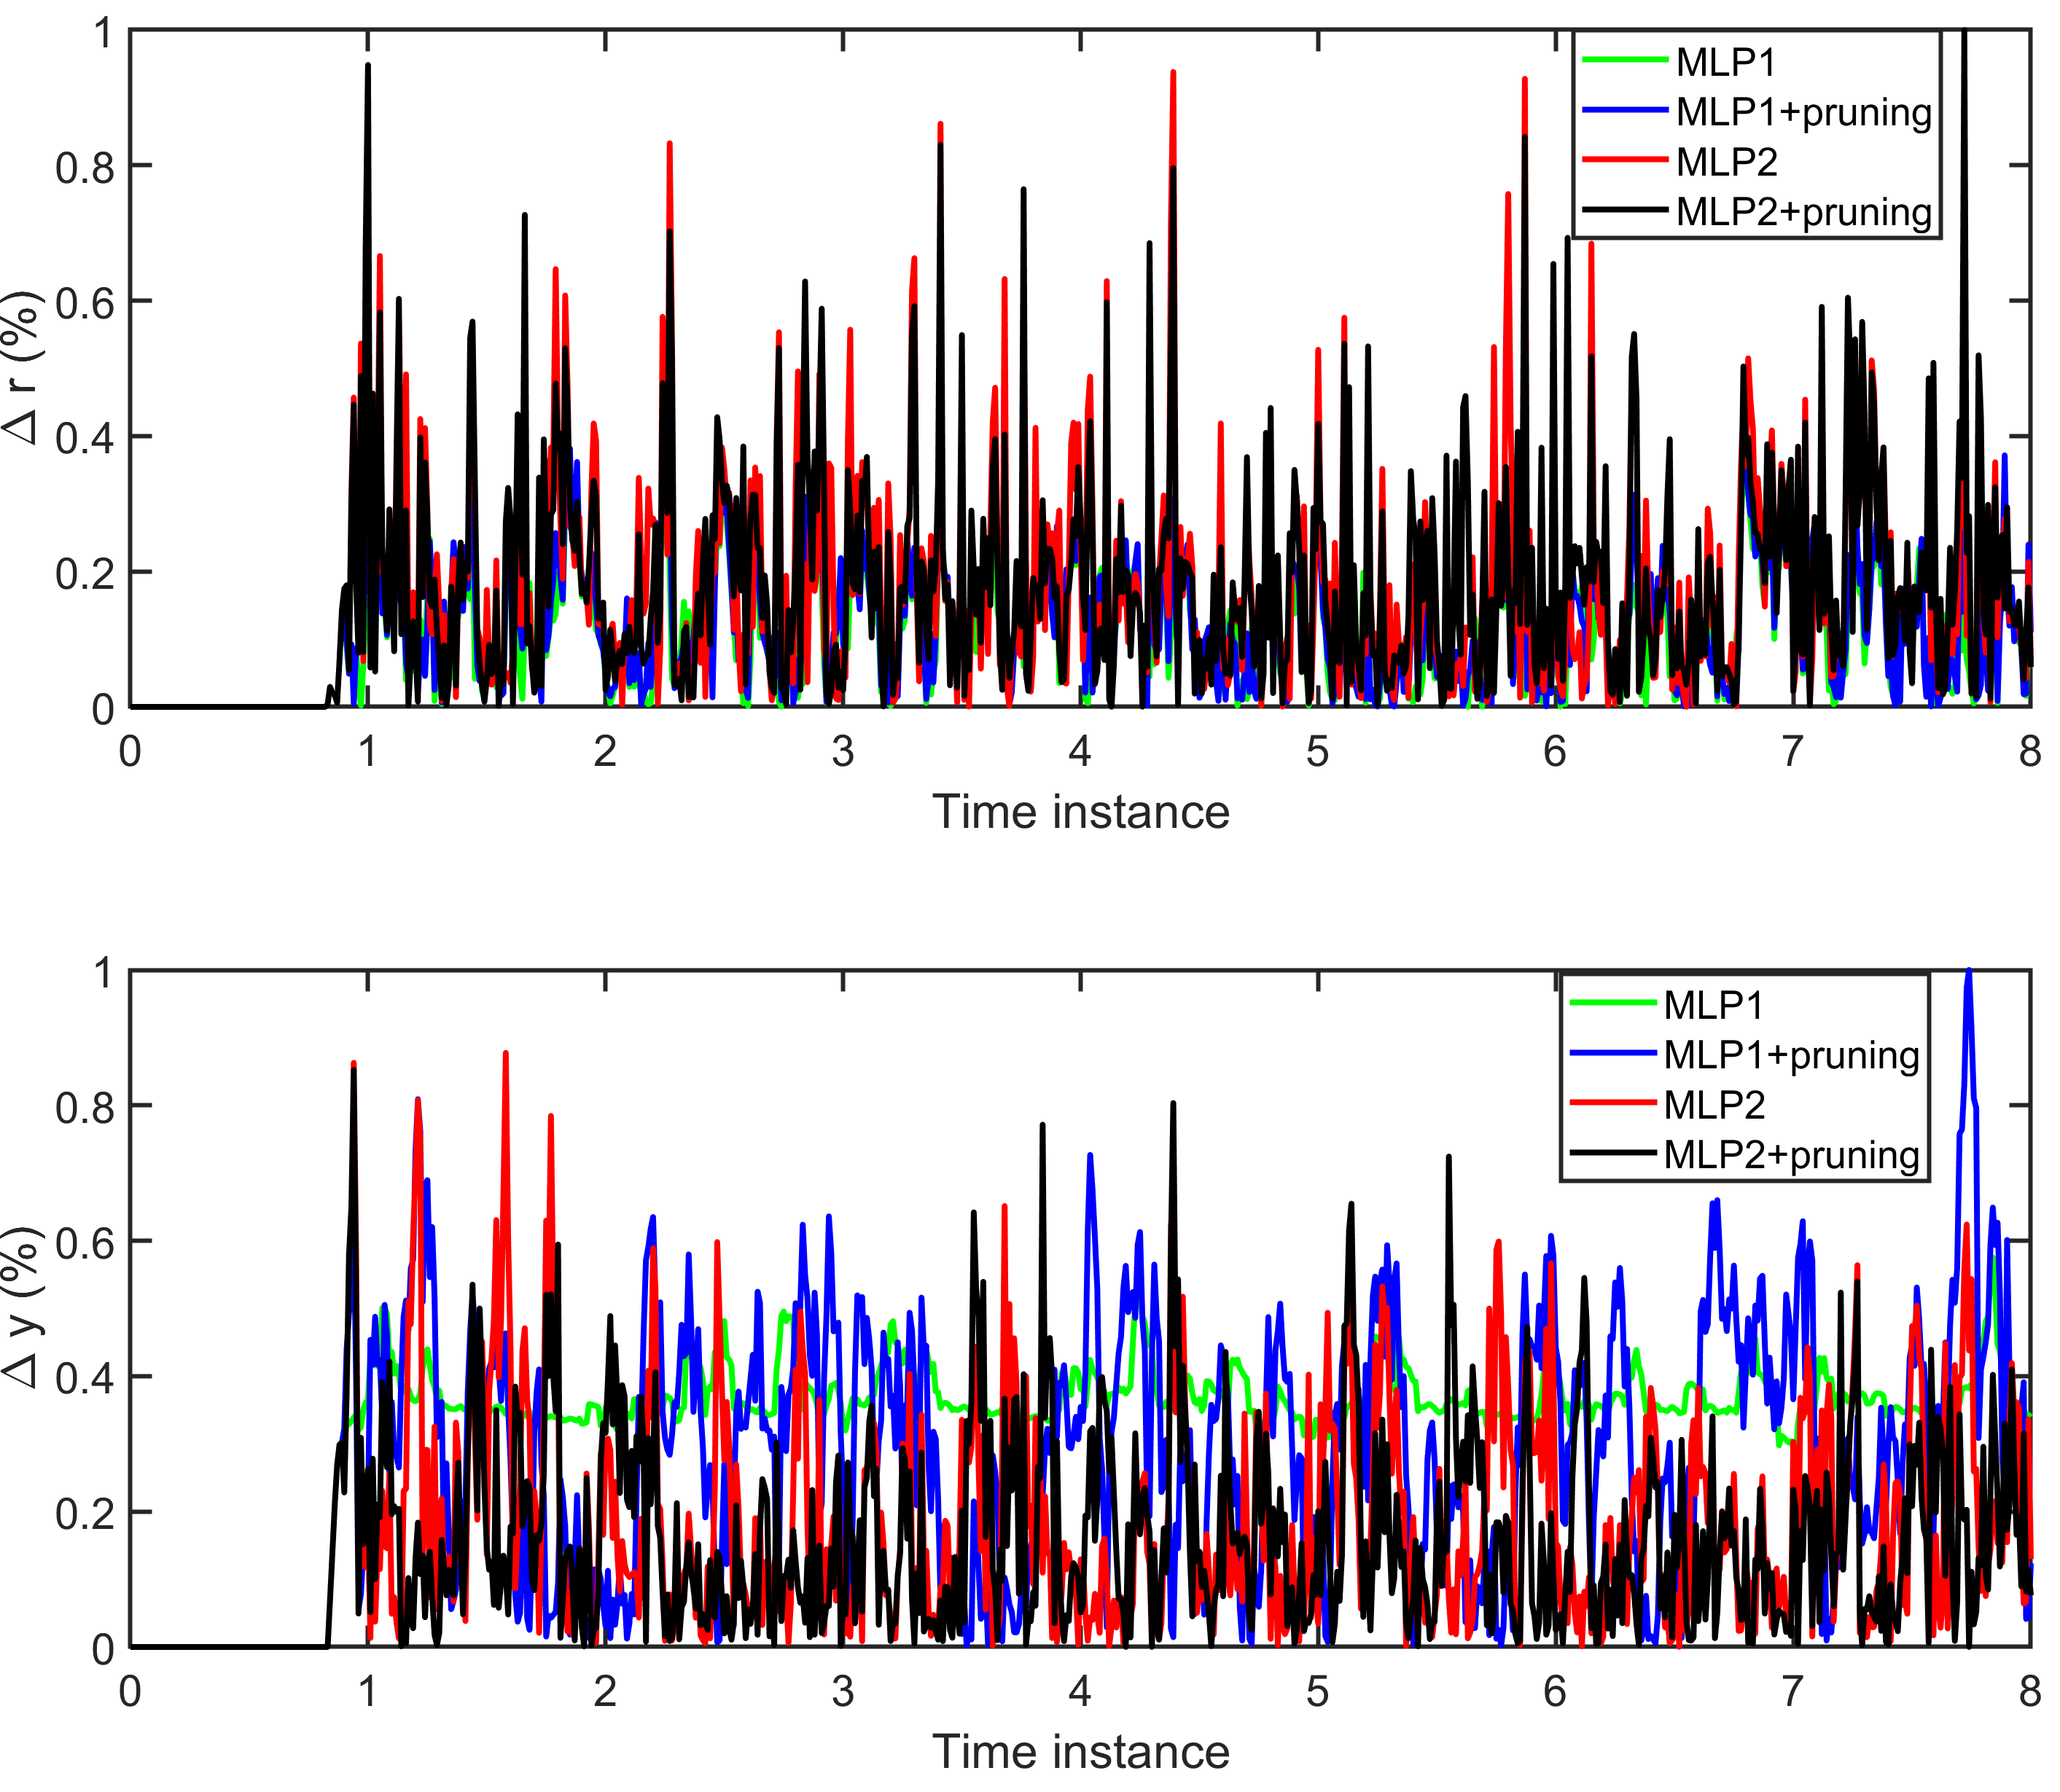
\includegraphics[scale=0.11]{new_sim_image/time-domain.png}
    \caption{Time-domain resilient KF results for four localization strategies under the attack scenario of Fig.~\ref{fig:generator_test_example_1}.}
    \label{fig:time_domain_result}
\end{figure}


\section{Conclusion} \label{sec:conclusion}
This paper developed a resilient estimation architecture that combines a Kalman filter, chi-square innovation monitoring, physics-guided attack generation, and channel-wise localization. The attack generator was formulated using finite-horizon maps that retain the dynamics of both the estimator and the controlled plant. This construction gives a detector-calibrated measure of stealthiness through the noncentral chi-square distribution, rather than through an unnormalized residual threshold.

The localization output was converted into an estimator input through calibrated safety probabilities. Under explicit calibration and conditional-independence assumptions, the selected subset is attack-free with a prescribed probability. The analysis further showed that attack sparsity limits the existence of a clean observable subset, while the size of the selected subset determines the conditional Kalman-filter covariance through the Riccati equation. The water-distribution case study demonstrated the empirical sensing redundancy and the localization improvement obtained by augmenting the training set with physics-guided attacks. Closed-loop numerical validation of the revised KF/$\chi^2$ architecture is outside the scope of the available data and is not inferred from the earlier residual-based results.

Future work will consider dependent channel-calibration models, time-varying sensor subsets, and unconditional error guarantees obtained by combining probabilistic selection with a robust update on the selection-failure event.


\iffalse
\section{Acknowledgements}
This material is based upon work supported by the Department of Energy under Award Number DE-CR0000005
\fi


\bibliographystyle{IEEEtran} 
\bibliography{IEEEabrv,mybib}


% if have a single appendix:
\iffalse
\appendix[System dynamics]  \label{sec:appendix}
The dynamics of the water distribution system \eqref{equ:water_level_adjustment} is given by


\begin{strip}
\begin{align*}
    A &=\resizebox{1\hsize}{!}{$\begin{bmatrix}
    0.994901337 & 0 & 0 & 0 & 0 & 0& 0 & 0& 0 &0\\
    0.001860443	& 0.994876876 & 0 & 0 & 0 & 0& 0 & 0& 0 &0 \\
    0 & 0.001859915& 0.994337441 & 0 & 0 & 0& 0 & 0& 0 &0 \\
    0 & 0 & 0.001859582 & 0.994519894 & 0 & 0 & 0& 0 & 0& 0 \\
    0 & 0 & 0& 0.001860036	& 0.994823733 & 0 & 0 & 0& 0 & 0 \\
    0 & 0 & 0 & 0 &	0.001860036	& 0.994520064 & 0 & 0 & 0& 0 \\
    0 & 0 & 0 & 0 & 0&  0.001860076 & 0.994865618 & 0 & 0 & 0\\
    0 & 0 & 0 & 0 & 0 &0 & 0.001860485 & 0.994957781 & 0 & 0 \\
    0 & 0 & 0 & 0 & 0 &0 &0 & 0.001859831 & 0.994166369 & 0 \\
    0 & 0 & 0 & 0 & 0 &0 & 0 &0 & 0.001859361 & 0.994454872
\end{bmatrix}$}, \\
B &= \resizebox{1\hsize}{!}{$\begin{bmatrix}
    0.009834083 & -0.008428458 & 0 & 0 & 0 & 0& 0 & 0& 0 &0\\
    0 & 0.009361412 & -0.008428355 & 0 & 0 & 0 & 0& 0 & 0& 0 \\
    0& 0 & 0.009131773 & -0.008426076 & 0 & 0 & 0& 0 & 0& 0 \\
    0 &0 & 0 & 0.009596549 & -0.008426847 & 0 & 0 & 0& 0 & 0\\
    0 & 0 & 0& 0& 0.009724914 & -0.00842813 & 0 & 0 & 0& 0 \\
    0 & 0 & 0 & 0 & 0 & 0.009942626 & -0.008426847 & 0 & 0 & 0 \\
    0 & 0 & 0 & 0 & 0& 0& 0.007972646 & -0.008428307 & 0 & 0\\
    0 & 0 & 0 & 0 & 0 &0 &0 & 0.009698484 & -0.008428697 & 0  \\
    0 & 0 & 0 & 0 & 0 &0 &0 & 0 & 0.009190367 & -0.008425353  \\
    0 & 0 & 0 & 0 & 0 &0 & 0 &0 & 0 & 0.009944375
\end{bmatrix}$},\\
C &= \begin{bmatrix}
   I_{10} &
C_1.^{\top}& C_2.^{\top}&C_3.^{\top}&C_4.^{\top}
\end{bmatrix}^{\top},
\end{align*}

$$ C_1 = \begin{bmatrix} 1 & -1 & 0 & 0 & 0 & 0& 0 & 0& 0 &0\\
    0 & 1 & -1 & 0 & 0 & 0& 0 & 0& 0 &0 \\
    0 & 0 & 1 & -1 & 0 & 0& 0 & 0& 0 &0 \\
    0 & 0 & 0 & 1 & -1 & 0 & 0& 0 & 0& 0 \\
    0 & 0 & 0& 0 & 1 & -1 & 0 & 0& 0 & 0 \\
    0 & 0 & 0 & 0 & 0 & 1 & -1 & 0 & 0& 0 \\
    0 & 0 & 0 & 0 & 0&  0 & 1 & -1 & 0 & 0\\
    0 & 0 & 0 & 0 & 0 &0 & 0 & 1 & -1 & 0 \\
    0 & 0 & 0 & 0 & 0 &0 &0 & 0 & 1 & -1 \end{bmatrix}, \hspace{2mm}
    C_2 =  \begin{bmatrix} 1 & 0 & -1 & 0 & 0 & 0& 0 & 0& 0 &0\\
    0 & 1 & 0 & -1 & 0 & 0& 0 & 0& 0 &0 \\
    0 & 0 & 1 & 0 & -1 & 0& 0 & 0& 0 &0 \\
    0 & 0 & 0 & 1 & 0 & -1 & 0& 0 & 0& 0 \\
    0 & 0 & 0& 0 & 1 & 0 & -1 & 0& 0 & 0 \\
    0 & 0 & 0 & 0 & 0 & 1 & 0 & -1 & 0& 0 \\
    0 & 0 & 0 & 0 & 0&  0 & 1 & 0 & -1 & 0\\
    0 & 0 & 0 & 0 & 0 &0 & 0 & 1 & 0 & -1\end{bmatrix},
$$


$$ C_3 =  \begin{bmatrix} 1 & 0 & 0 & -1 & 0 & 0& 0 & 0& 0 &0\\
    0 & 1 & 0 & 0 & -1& 0& 0 & 0& 0 &0 \\
    0 & 0 & 1 & 0 & 0 & -1& 0 & 0& 0 &0 \\
    0 & 0 & 0 & 1 & 0 & 0 & -1& 0 & 0& 0 \\
    0 & 0 & 0& 0 & 1 & 0 & 0& -1& 0 & 0 \\
    0 & 0 & 0 & 0 & 0 & 1 & 0 & 0 & -1& 0 \\
    0 & 0 & 0 & 0 & 0&  0 & 1 & 0 & 0 & -1\end{bmatrix}, \hspace{2mm}
    C_4 =  \begin{bmatrix} 1 & 0 & 0 & 0 & -1 & 0& 0 & 0& 0 &0\\
    0 & 1 & 0 & 0 & 0& -1& 0 & 0& 0 &0 \\
    0 & 0 & 1 & 0 & 0 & 0& -1 & 0& 0 &0 \\
    0 & 0 & 0 & 1 & 0 & 0 & 0& -1 & 0& 0 \\
    0 & 0 & 0& 0 & 1 & 0 & 0& 0& -1 & 0 \\
    0 & 0 & 0 & 0 & 0 & 1 & 0 & 0 & 0& -1\end{bmatrix}.
$$
\end{strip}

\fi
% or
%\appendix  % for no appendix heading
% do not use \section anymore after \appendix, only \section*
% is possibly needed

% use appendices with more than one appendix
% then use \section to start each appendix
% you must declare a \section before using any
% \subsection or using \label (\appendices by itself
% starts a section numbered zero.)
%


% Can use something like this to put references on a page
% by themselves when using endfloat and the captionsoff option.
\ifCLASSOPTIONcaptionsoff
  \newpage
\fi



% trigger a \newpage just before the given reference
% number - used to balance the columns on the last page
% adjust value as needed - may need to be readjusted if
% the document is modified later
%\IEEEtriggeratref{8}
% The "triggered" command can be changed if desired:
%\IEEEtriggercmd{\enlargethispage{-5in}}

% references section

% can use a bibliography generated by BibTeX as a .bbl file
% BibTeX documentation can be easily obtained at:
% http://mirror.ctan.org/biblio/bibtex/contrib/doc/
% The IEEEtran BibTeX style support page is at:
% http://www.michaelshell.org/tex/ieeetran/bibtex/
%\bibliographystyle{IEEEtran}
% argument is your BibTeX string definitions and bibliography database(s)
%\bibliography{IEEEabrv,../bib/paper}
%
% <OR> manually copy in the resultant .bbl file
% set second argument of \begin to the number of references
% (used to reserve space for the reference number labels box)
% \begin{thebibliography}{1}

%\bibitem{IEEEhowto:kopka}
%H.~Kopka and P.~W. Daly, \emph{A Guide to \LaTeX}, 3rd~ed.\hskip 1em plus
%  0.5em minus 0.4em\relax Harlow, England: Addison-Wesley, 1999.

%\end{thebibliography}

% biography section
% 
% If you have an EPS/PDF photo (graphicx package needed) extra braces are
% needed around the contents of the optional argument to biography to prevent
% the LaTeX parser from getting confused when it sees the complicated
% \includegraphics command within an optional argument. (You could create
% your own custom macro containing the \includegraphics command to make things
% simpler here.)
%\begin{IEEEbiography}[{\includegraphics[width=1in,height=1.25in,clip,keepaspectratio]{mshell}}]{Michael Shell}
% or if you just want to reserve a space for a photo:
\iffalse
\begin{IEEEbiography}{Yu Zheng (Student Member, IEEE)}
received his B.S. in marine engineering from Wuhan University of Technology, China, in 2017, and his M.S. degree in marine and automatic engineering from Huazhong University of Science and Technology, China, in 2019. He is currently a Ph.D candidate of Department of Electrical and Computer Engineering at Florida state University. His research interest is around concurrent model resilient control and estimation.
\end{IEEEbiography}

% if you will not have a photo at all:
\begin{IEEEbiography}{Ali Sayghe(Student Member, IEEE)}
received his B.S. and M.S in Electronic Engineering Technology from Arizona State University, Tempe, Arizona, in 2010, 2013. He is currently a Ph.D. candidate in the Department of Electrical and Computer Engineering at Florida State University. His research interest is around Power system security and control.
\end{IEEEbiography}

% insert where needed to balance the two columns on the last page with
% biographies
%\newpage

\begin{IEEEbiography}{Olugbenga Moses Anubi (Senior Member, IEEE)}
is an Assistant Professor in the Electrical and Computer Engineering Department at the Florida State
University (FSU), with affiliations with the Center
for Advanced Power Systems (CAPS) and the Center
for Intelligent Systems, Controls and Robotics (CISCOR). He received a Ph.D in Mechanical Engineering, from the University of Florida. Prior to joining
FSU, he was a Lead Control Systems Engineer at GE
Global Research, NY. His work within GE resulted
in 12 Patent Applications and several recognitions
including the GE Technology Award (Physical+Digital), the Connected Controls Technical Achievement Award, the Whitney Award and the Dushman
Technology Award. His research interests include robust, resilient and adaptive
control systems, real-time optimization , robotics, and vehicle dynamics \& control.
\end{IEEEbiography}
\fi
% You can push biographies down or up by placing
% a \vfill before or after them. The appropriate
% use of \vfill depends on what kind of text is
% on the last page and whether or not the columns
% are being equalized.

%\vfill

% Can be used to pull up biographies so that the bottom of the last one
% is flush with the other column.
%\enlargethispage{-5in}



% that's all folks
\end{document}


